\chapter{Network Measurements}
\label{chp:measurements2}


\noindent This chapter will display the experiments carried out concerning data sending rate from the \gls{nRF52} to the \gls{Raspberry Pi}. The goal is to determine the most efficient combination of the amount of data to send in one transmission. We will discuss sending frequency, \gls{payload} size and protocols to use in the different scenarios. 

\section{Description of measurements}

\noindent The following sections will discuss if \textit{fragmentation} is a major issue when sending data through low energy networks. Another point will be which of the protocols described in chapter \ref{chp:background} is the most efficient to use when the goal is to get a maximum amount of \gls{payload} compared to the total throughput. Data will be sent through the network, containing a payload of constant length. Wireshark will be a central part of the measurements presented, and the packet size will be increased to see the changes. These problems are essential in the discussion of objective O.4. %\todo{Denne sectionen sier for mange tanker paa en gang!}

\noindent Before the experiment started, our expected result was that sending a small amount of data at a time would not be preferable, because of the needed bytes to set up the connection, header files and so on. We did not know the packet size needed before it would be considered profitable to send them regarding the cost of energy and network capacity. This is dependent on the situation where the network will be used. A system with sensors to analyse real-time patient data to see if a patient is in a stable state needs to be reliable, and the data will be sent no matter if it is profitable for the network or not. In this case, timing is the most important. A system used in a company to monitor how many cups of coffee are brewed during a day can easily store data in the end node and send larger amounts of data less frequently, if this is profitable for the network. 

\noindent When sending \gls{ble} packets over the network, observations from the system show that the maximum packet size is 31 bytes in the testbed. Each of these packages needs a header field of 4 bytes, meaning 27 bytes left for useful data. However, to start the connection at all, 76 bytes are needed, meaning three \gls{ble} packets. The ratio between \textit{useful} and \textit{needed} data transferred start out very poorly if the payload sent is tiny. The best possible ratio of useful data we can achieve will also be limited by this. 27 bytes \gls{payload} and 4 bytes header field is 87,1 \%, calculated in the following equation: 
 %\todo{If we ignore con start?}

\begin{equation} \label{percentageHeader}
    lim_{x\to\infty} \frac{x + 27}{x + 31 + C} = \frac{27 \, byte}{31 \, byte}*100 \, \approx 87,1 \,\%
\end{equation} 

%\todo{Tjaa, ikke helt enig? Forklar bedre at det er header?}


\noindent During measurements in the physical testbed, the actual result will probably be considerably lower than this because \gls{6lowpan} and \gls{coap} packets could require some additional fields for each packet. There are also other additional protocols in \gls{ble} that will require some packets, like the occasional \glspl{ack} from ACL. It is also logical to expect some other disturbing factors in a real-world wireless network. 

\section{Possible limitations in the network}

\subsection{Stable transfer rate}

\noindent As soon as the end nodes of the network could communicate with the Raspberry Pi using \gls{coap}, the next step was to test the transfer rate of the connection. To measure the network transfer rate, \textit{ping6} was used. This is a software tool used to test networks using \gls{ipv6} in a network. Results from these measurements are being shown as \textit{ms} used for every \acrlong{rtt}. 

\begin{verbatim}
ping6 2001::2e6:6aff:fe64:54dd
ping6 google.com
\end{verbatim}

%\begin{figure}[h!]
%    \centering
%    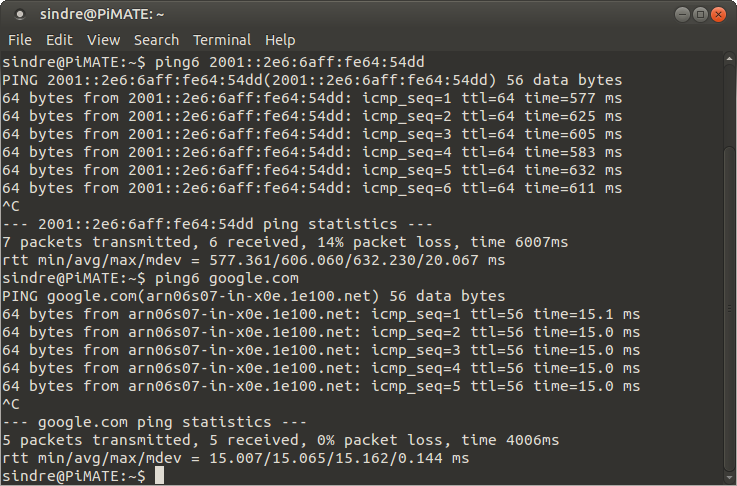
\includegraphics[width=1.0\textwidth]{ping6test.png}    
%    \caption{Comparison: ping nRF52 and ping google.com}
%    \label{fig:pingComparison}
%\end{figure}


\noindent To receive messages using \gls{con}, a \gls{coap} GET-message is sent from a requesting client. As soon as the response has been received at the client-side, another GET message is being sent, which means there is always either a GET-message or a message containing a \gls{payload} in the network, given that the end node has a sensor connected that provides streaming data. 

\noindent In \gls{non}, there are two different options. A new message can be sent when the set field \textit{Max-Age} has expired, which tells the number of seconds the device should wait before sending a new packet \cite{shelby2014constrained}. The other choice is to send a new message every time a given field has been updated. This would have been the best solution in the testbed, but it was never possible to update this field using accelerometer data, as expected in this case. The only choice was to set the Max-Age to 1 second, which was the lowest setting leading to a stable . This gives a stable and reliable transfer frequency at 1 second, even though this is a limitation compared to the sending frequency in \gls{con}. After a test period, it was therefore decided that the best solution for \gls{non} would be to gather data from sensors at a higher rate, and store them in the \gls{nRF52} temporary. Every second all the measured values are being transferred to the \gls{Raspberry Pi}, the temporarily values are deleted, and the measurement continues. This method has proven to be a stable solution, with successful tests over several days. \gls{con} can handle more frequent transportations than this in this system, on average four times per second. See the test shown in chapter \ref{chp:measurements2}.6. Figure  \ref{fig:CoAPNONwiresharkSetUp} shows the initial set up of a \gls{non}-connection, where the stable transfer rate of one second can be seen at the timestamps at the bottom of the figure. 

%\begin{equation} \label{avg_eq}
%    \overline{x}_{n} = \frac{\sum\limits_{i=1}^n x_{i}}{n}
%\end{equation}

%Equation \ref{avg_eq} shows the standard way used to calculate an average of the measured values. Here \textit{a} is any real number and \textit{n} is any integer. 

%After a test period, the problems explained in was fixed. A more reliable test could then be performed, as shown in figure \ref{fig:ping2}. Using equation \ref{avg_eq} to calculate average gives 


\noindent Results from these first tests gave an approximate average of 250 \textit{ms} \gls{rtt}, from a request is sent to the response is received. The standard deviation in these cases was on average $ \sigma = 25 \, ms $, which is a variation of 10 \%. In total ten different measurements at different time were performed, an example can be seen in figure \ref{fig:ping3}. These measurements were performed using different versions of \glspl{nRF52}, and a different amount of these devices connected to the central Raspberry Pi at once. This is considered quite slow in such a system, and way beneath the transfer limitations of both \gls{ble}, \gls{6lowpan} and \gls{coap}. Another factor could be the limited power supply and computational power, but it is not clear what is the main cause at this point. This will regardless be a major limitation in the network.
%, as explained in chapter \ref{chp:background}. 
%\todo{Tja, staar det noe i background egentlig?}
%\todo{Explain limitations more clear?}

\begin{figure}[ht]
    \centering
    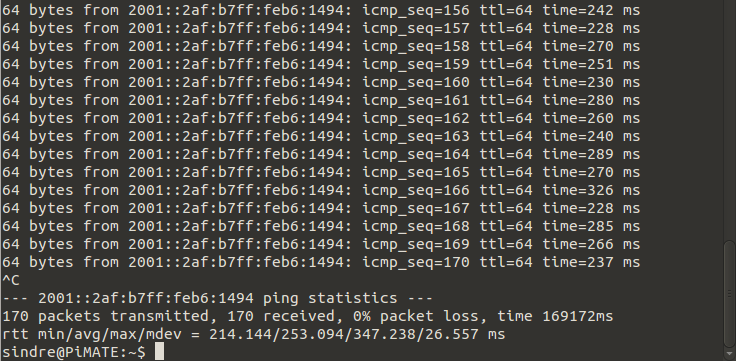
\includegraphics[width=1.0\textwidth]{ping4.png}    
    \caption{Ping nRF52 from Raspberry Pi}
    \label{fig:ping3}
\end{figure}


\noindent The conclusion from these initial tests is therefore that \gls{coap} \gls{con} can be used at a lower transfer interval than \gls{coap} \gls{non} in the testbed. \gls{con} can in best case send a message every 250 \textit{ms}, which is as expected compared to the high \gls{rtt} measured in this network. An example of one of the \gls{rtt} tests can be seen in figure \ref{fig:ping3}. \gls{non} has shown the same results regarding \gls{rtt}, but the connection has in general been more unstable in the initial tests, even though Max-Age means data can only be sent every second. From this starting point it is expected that \gls{con} can send a larger \gls{payload} per second for small \glspl{payload}, but \gls{non} require less of the network to send each message. In addition it is expected that \gls{non} will get a higher percentage of \gls{payload} compared through the total throughput for larger \glspl{payload}, since no \glspl{ack} are required in this solution. 



\subsection{Packet fragmentation}

\noindent In Internet Routing, fragmentation is known as the action of splitting data into smaller \glspl{packet}, to satisfy the maximal limits of the different technologies or protocols used (e.g. \gls{ble} and \gls{6lowpan} in the testbed). Each of these packets needs header fields of a certain size, or other requirements. In a network of \glspl{microcontroller}, fragmentation can be a factor that needs to be taken into account to optimize the \gls{payload} sent through the system. To better understand fragmentation, imagine a train with carriages as shown in Figure \ref{fig:trainExample}. 

\begin{figure}[ht]
    \centering
    \includegraphics[width=0.9\textwidth]{tooog.png}    
    \caption{Packet fragmentation -- train comparison}
    \label{fig:trainExample}
\end{figure}

\noindent To be able to operate at all, the train needs a locomotive with an engine driver, a conductor and a cafe carriage. As soon as these things are already there, the company owning the train gets better and better off for every passenger buying a ticket. Lets assume that every carriage can carry 4 employees and 27 passengers, to make it directly comparable to the \gls{ble} packets in the network. Eventually all the carriages will be full, and a decision has to be made if it will be profitable to fit another carriage. It will in general be most profitable to use as many carriages as the locomotive can handle, and to fill up every carriage as much as possible. It will however not be a good idea to connect another carriage if there will only be one additional passenger sitting there, since the extra weight of the carriage adds unnecessary additional weight to the train set compared to the income. 

\noindent In this example, the locomotive and employees are the \gls{6lowpan} packet, that are needed no matter what to get the train working. Each additional carriage is a \gls{ble} packet. The goal is therefore to find the maximal number of passengers compared to the cost of adding additional carriages, in other words the maximum number of bytes compared to the number of sent packets. This is known as fragmentation, fragmenting data into smaller pieces to satisfy the maximal limitations of packet sizes in the different protocols. This can be exploited by a system developer to maximize the percentage of \gls{payload} compared to \gls{throughput} in the network.
 
\newpage

\section{Measurements}

\subsection{CoAP CON}

\noindent As previously explained, \gls{coap} can be split into two different main sections. \gls{con} messages can in the testbed be sent quite frequently, but every message needs to get an \gls{ack} before the next message can be sent. This means that it has the possibility of being quite fast, but several extra packets needs to be transported through to get usable data at the other end of the link. The other alternative is \gls{non}, where each message does not need an \gls{ack}. 


%\begin{figure}[ht]
%    \centering
%    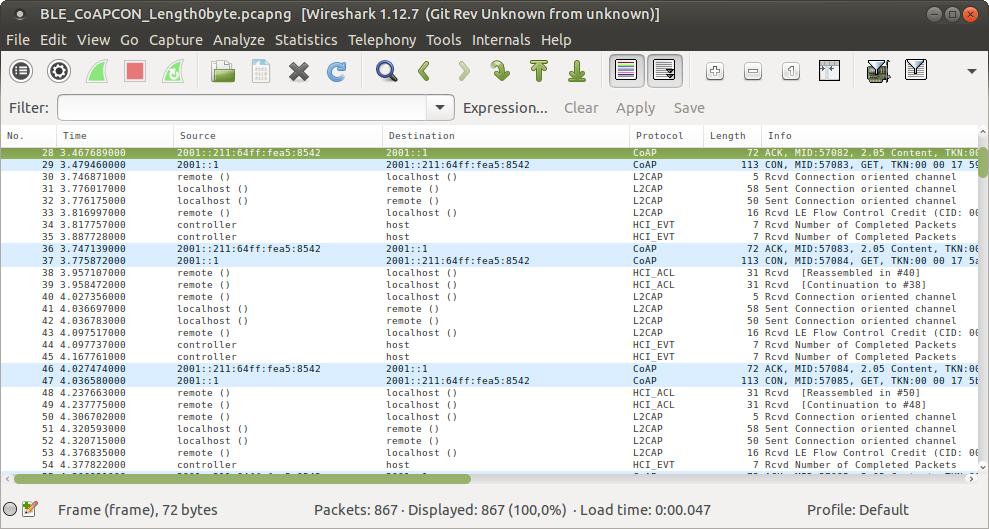
\includegraphics[width=\textwidth]{wiresharkCoAPCON0byte.png}    
%    \caption{Wireshark capture, CoAP CON, 0 bytes goodput}
%    \label{fig:coapCON0Wireshark}
%\end{figure}



%\begin{figure}[ht]
%    \centering
%    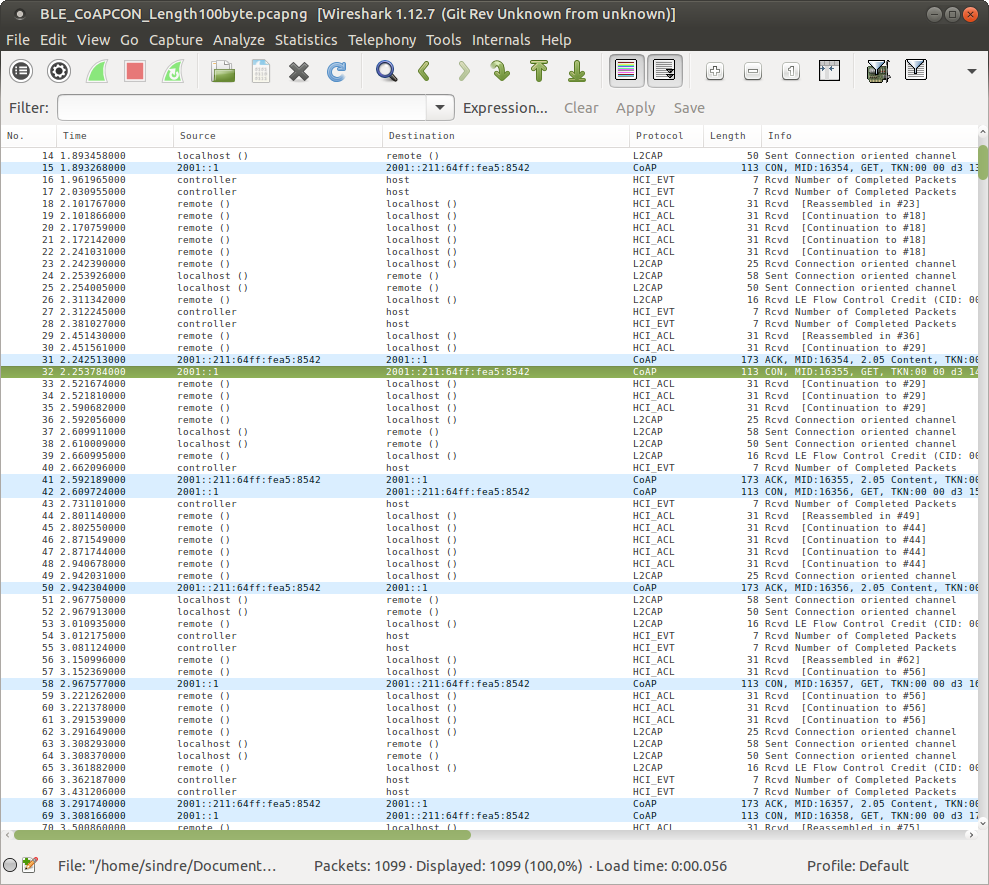
\includegraphics[width=\textwidth]{wiresharkCON100bytes.png}    
%    \caption{Wireshark capture, CoAP CON, 100 bytes goodput}
%    \label{fig:coapCON100Wireshark}
%\end{figure}

\noindent In \textit{Wireshark} it is possible to display all captured packets, or filter packets regarding what protocol they are using (e.g. \gls{tcp} or \gls{coap}). The following examples will only focus on packets sent using \gls{coap} in addition to capturing all bluetooth packets. This will show how the fragmentation of \gls{coap} packets needs to be done in order to fit into the size of \gls{ble} packets. When measuring packet sizes concerning fragmentation of the network, all measurements of the same constant \gls{payload} gave the same result, since fragmentation is being handled the same way every time. These examples are therefore taken from one of the experiments, even though several where done\footnote{All the measured data can be found on \url{https://www.github.com/sische/MasterThesis}}. 

\begin{table}[ht]
\centering
\caption{Wireshark CoAP CON 0 bytes payload}
\label{coapCON0table}
\begin{tabular}{lllll}
Number & Time   & Protocol & Length & Info                             \\ \hline
36     & 3.7471 & CoAP     & 72     & ACK, MID:57083, 2.05 Content     \\
37     & 3.7759 & CoAP     & 113    & CON, MID:57084, GET              \\
38     & 3.9571 & HCI\_ACL & 31     & Rcvd {[}Reassembled in \#40{]}   \\
39     & 3.9584 & HCI\_ACL & 31     & Rcvd {[}Continuation to \#38{]}  \\
40     & 4.0274 & L2CAP    & 5      & Rcvd Connection oriented channel \\
41     & 4.0367 & L2CAP    & 58     & Sent Connection oriented channel \\
42     & 4.0368 & L2CAP    & 50     & Sent Connection oriented channel \\
43     & 4.0975 & L2CAP    & 16     & Rcvd LE Flow Control             \\
44     & 4.0977 & HCI\_EVT & 7      & Rcvd Number of Completed Packets \\
45     & 4.1678 & HCI\_EVT & 7      & Rcvd Number of Completed Packets \\
46     & 4.0275 & CoAP     & 72     & ACK, MID:57084, 2.05 Content     \\
47     & 4.0366 & CoAP     & 113    & CON, MID:57085, GET              \\ \hline
\end{tabular}
\end{table}

\noindent Table \ref{coapCON0table} shows the most basic example of a capture of packets in Wireshark using \gls{con}. The full capture can be seen in the Appendix \ref{chp:appendixb}. In this case an empty \textit{char} array was sent, meaning a \gls{payload} equal to 0 byte. As a consequence, all the captured bytes correspond solely to data sent by the network protocols. The 31 bytes per \gls{ble} packet, the maximum for \gls{ble} in the system, have been exceeded twice. Therefore, three packets were needed. The first packet is labeled \textit{[Reassembled in \#40]}, the second \textit{[Continuation to \#38]} and the last \textit{Connection oriented channel}. Then the \gls{ack} packages follows, two packages of 58 and 50 bytes, respectively. A final pair of packets tells how many packages were completed, as a built in feature in \gls{ble}  \gls{hci}  and \gls{acl}. All of these packages can fit into one \gls{6lowpan} packet, since the total number of bytes are less than 270 bytes. %\todo{Say 0\% goodput somewhere in here?}




\begin{table}[H]
\centering
\caption{Wireshark CoAP CON 100 bytes payload}
\label{coapCON100table}
\begin{tabular}{lllll}
Number & Time   & Protocol & Length & Info                             \\ \hline
29     & 2.4514 & HCI\_ACL & 31     & Rcvd {[}Reassembled in \#36{]}   \\
30     & 2.4516 & HCI\_ACL & 31     & Rcvd {[}Continuation to \#29{]}  \\
31     & 2.2425 & CoAP     & 173    & ACK, MID:16354, 2.05 Content     \\
32     & 2.2538 & CoAP     & 113    & CON, MID:16355, GET              \\
33     & 2.5217 & HCI\_ACL & 31     & Rcvd {[}Continuation to \#29{]}  \\
34     & 2.5218 & HCI\_ACL & 31     & Rcvd {[}Continuation to \#29{]}  \\
35     & 2.5907 & HCI\_ACL & 31     & Rcvd {[}Continuation to \#29{]}  \\
36     & 2.5921 & L2CAP    & 25     & Rcvd Connection oriented channel \\
37     & 2.6099 & L2CAP    & 58     & Sent Connection oriented channel \\
38     & 2.6100 & L2CAP    & 50     & Sent Connection oriented channel \\
39     & 2.6610 & L2CAP    & 16     & Rcvd LE Flow Control             \\
40     & 2.6621 & HCI\_EVT & 7      & Rcvd Number of Completed Packets \\
41     & 2.5922 & CoAP     & 173    & ACK, MID:16355, 2.05 Content     \\
42     & 2.3097 & CoAP     & 113    & CON, MID:16356, GET              \\ 
43     & 2.7311 & HCI\_EVT & 7      & Rcvd Number of Completed Packets \\ \hline
\end{tabular}
\end{table}

\noindent In table \ref{coapCON100table}, 100 bytes of \gls{payload} is being sent through the network using \gls{con}. The same basic packages are still needed there, but in addition 100 bytes of data is added. This means adding more \gls{ble} packets, but also that the percentage of useful data sent through is  higher, approximately 34 \% in this case, as seen in equation \ref{eqCON100byte2}. By doing several experiments like this, it was possible to create the graph in Figure \ref{fig:coapCON0200}. This shows the correlation between \gls{payload} and \gls{throughput} compared to the number of packets sent, measured every 10th byte from 0 byte to 200 bytes large packets. %Several tests have been performed to test the fragmentation of packets, which show that the fragmentation is always done the same way for a \gls{payload} of a fixed size. The packet sizes therefore take one of the measurements as a point of referance \footnote{All the measured data can be found on \url{https://www.github.com/sische/MasterThesis}}.

 
%\begin{equation} \label{eqCON100byte1}
%    \frac{100 \, byte \, goodput}{173 \, byte \, throughput + \, 113 \, byte \, ack}*100 \, %\approx 35 \,\%
%\end{equation}

\begin{equation} \label{eqCON100byte2}
    \frac{100 \, byte \, goodput}{180 \, byte \, throughput + \, 113 \, byte \, ack}*100 \, \approx 34 \,\%
\end{equation}


\begin{figure}[ht]
    \centering
    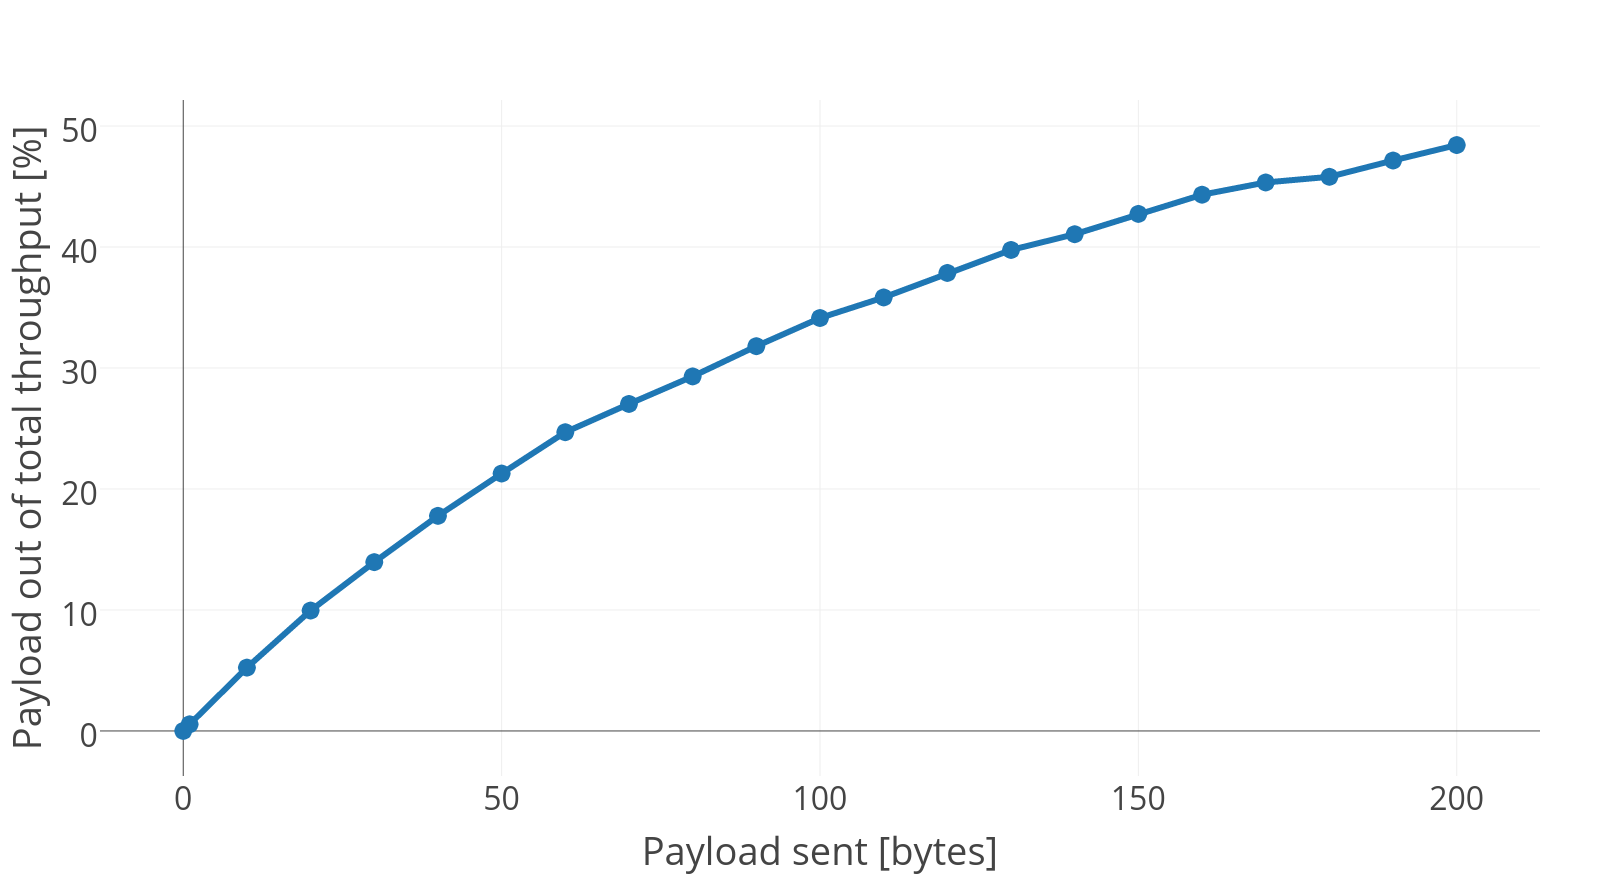
\includegraphics[width=1.0\textwidth]{CON0-200withAcks.png}    
    \caption{CoAP CON with ACKs, 0-200 bytes sent}
    \label{fig:coapCON0200}
\end{figure}

\noindent In this particular case shown in figure \ref{fig:coapCON0200}, it makes no sense to send less than 50 bytes of useful data at once, since more than 50 \% of the bytes sent will be header files. This is comparable to having a locomotive and full crew at disposal, but only a few or none paying passengers. The best possible result is to have every carriage full, with 27 passengers and 4 employees. Since at least 4 bytes out of every 31 sent needs to be used to header information, the best possible result will be 87,1 \%. In mathematics, this is described as a \textit{horizontal asymptote} since the distance between the graph and \textit{y = 87,1} will approach zero after an infinite number of bytes has been transferred, if the only limitation was \gls{ble} packets. In this network other limitations like \gls{6lowpan} header files needs to be considered as well. The graph will still approach 87,1 \%, which was calculated in equation \ref{percentageHeader}, just as the values climbing in figure \ref{fig:coapCON0200}, even before the \gls{payload} has reached 200 bytes.

\begin{equation} \label{percentage}
    \frac{100 \, byte \, goodput}{180 \, byte \, throughput + \, 113 \, byte \, ack}*100 \, \approx 34 \,\%
\end{equation}

%\begin{figure}[ht]
%    \centering
%    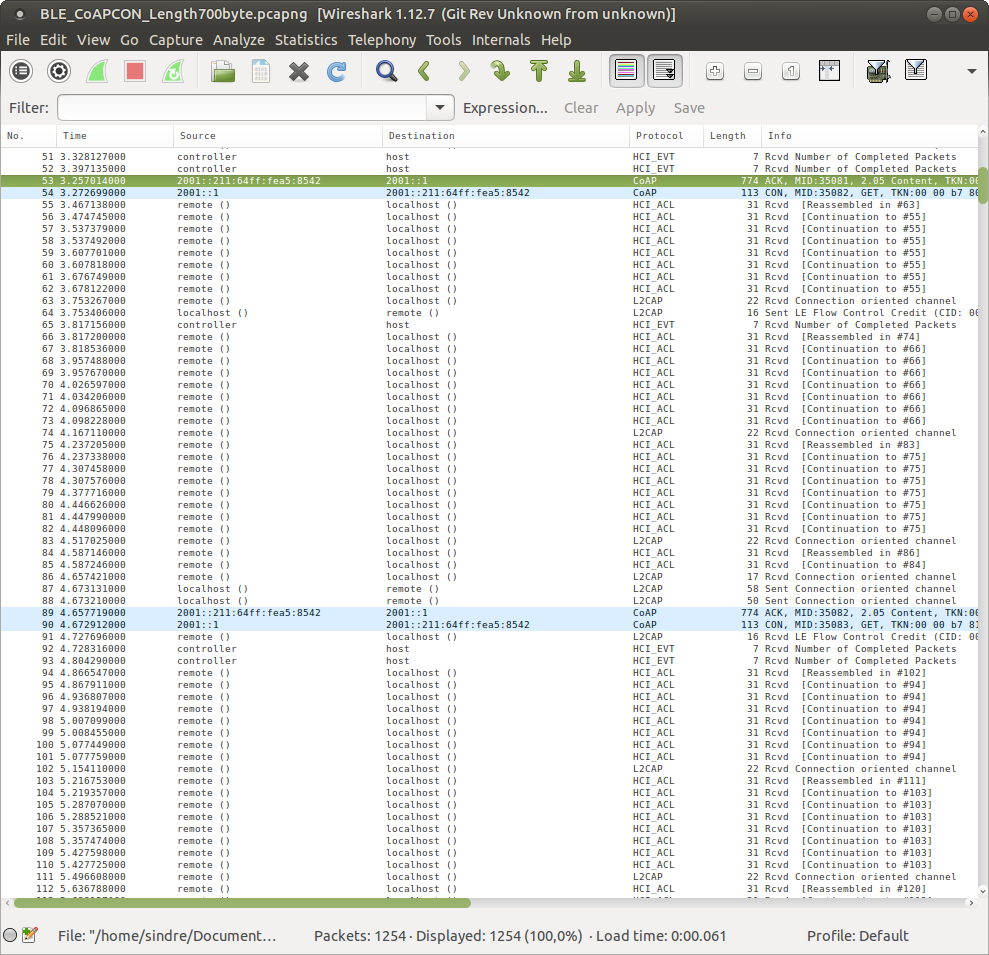
\includegraphics[width=\textwidth]{Wireshark700bytes2.png}    
%    \caption{Wireshark capture, CoAP CON, 700 bytes goodput}
%   \label{fig:coapCON700Wireshark}
%\end{figure}

%\newpage

\subsection{CoAP NON}

\noindent A \gls{coap} \gls{non} request does not require a response in form of an \gls{ack} to each \gls{coap} packet being sent. This means that the 108 bytes sent to and handled by the end node can be skipped. In the end nodes this leads to less computational power, and less network capacity is needed to transfer data both ways. This solution makes sense to use in networks where the system will still work as needed even if some packets are being dropped, since packets can be lost without the use of \glspl{ack}. As explained in chapter \ref{chp:measurements2}.1.1, the transfer frequency is limited using \gls{non} in this system, due to the use of Max-Age instead of GET-requests. The transfer rate is therefore set to one per second for this protocol. 

\begin{table}[ht]
\small
\centering
\caption{Wireshark CoAP NON 0 bytes payload}
\label{coapNON0table}
\begin{tabular}{lllll}
\hline
Number & Time    & Protocol & Length & Info                             \\ \hline
%\rowcolor{blue} 
90     & 23.0405 & HCI\_ACL & 31     & Rcvd {[}Reassembled in \#92{]}   \\
91     & 23.0411 & HCI\_ACL & 31     & Rcvd {[}Continuation to \#90{]}  \\
92     & 23.1107 & L2CAP    & 9      & Rcvd Connection oriented channel \\
93     & 23.1109 & CoAP     & 76     & NON, MID:14, 2.05 Content        \\ \hline
\end{tabular}
\end{table}


\noindent A basic example of the \gls{coap} \gls{non} connection is shown in table \ref{coapNON0table}\footnote{The entire Wireshark capture can be seen in Appendix \ref{chp:appendixb}}. This is directly comparable to table \ref{coapCON0table}, that shows a Wireshark capture of \gls{coap} \gls{con} packages. It is easy to see that a lot fewer packages needs to be sent using \gls{ble}, without the use of \glspl{ack}. The total amount of bytes sent is 31+31+9=71 bytes, meaning three \gls{ble} packages sent in one \gls{6lowpan} packet. \gls{con} has a packet size of 76 bytes in this transmission, which means a total of 5 header bytes and additional fields are needed. This is less than half of what was needed using \gls{coap} \gls{con}, where the 108 \gls{ack} packets were needed in addition. The packets are still recognizable the same way as before when captured in Wireshark. The first packet is labelled \textit{[Reassembled in \#40]}, the second \textit{[Continuation to \#38]} and the last \textit{Connection oriented channel}.

\noindent Fewer packets sent means less energy used in end nodes, less network capacity needed and less computational power in the end node. This approach will hopefully lead to a higher percentage of \gls{payload} compared to throughput. Therefore, tests were set up to measure this with \gls{payload} sizes between 0 and 200 bytes, measuring with an increasing interval of every 10 bytes. This will compare how the correlation between \gls{payload} and \gls{throughput} developed as the \gls{payload} size increased.

\begin{table}[H]
\small
\centering
\caption{Wireshark CoAP NON 100 bytes payload}
\label{coapNON100table}
\begin{tabular}{lllll}
\hline
Number & Time    & Protocol & Length & Info   							  \\ \hline                          
39     & 11.0363 & CoAP     & 177    & NON, MID:2, 2.05 Content         \\
40     & 11.9452 & HCI\_ACL & 31     & Rcvd {[}Reassembled in \#45{]}   \\
41     & 11.9465 & HCI\_ACL & 31     & Rcvd {[}Continuation to \#40{]}  \\
42     & 12.0154 & HCI\_ACL & 31     & Rcvd {[}Continuation to \#40{]}  \\
43     & 12.0168 & HCI\_ACL & 31     & Rcvd {[}Continuation to \#40{]}  \\
44     & 12.0857 & HCI\_ACL & 31     & Rcvd {[}Continuation to \#40{]}  \\
45     & 12.0858 & L2CAP    & 29     & Rcvd Connection oriented channel \\
46     & 12.0860 & CoAP     & 177    & NON, MID:3, 2.05 Content         \\ \hline
\end{tabular}
\end{table}

\noindent Table \ref{coapNON100table} shows the case where 100 bytes of data are sent using \gls{coap} \gls{non}. This is directly comparable to the test shown in table \ref{coapCON100table}, where the same amount of data is sent using \gls{con}. The overall structure is the same as before. Since it is only one packet noted \textit{Reassembled in \#n}, which marks the beginning of a new \gls{6lowpan} packet. The total amount sent must therefore be under 270 bytes, which makes sense. The \gls{non} packet size is here 177 bytes, compared to 173 bytes in \gls{con}, meaning that a \gls{non} packet require an additional header field of 4 bytes. Overall a small difference in the packets containing data, but as expected a lot more packets needs to be sent in total in \gls{con}. Using these measurements the following plot could be drawn. 

%\begin{figure}[ht]
%    \centering
%    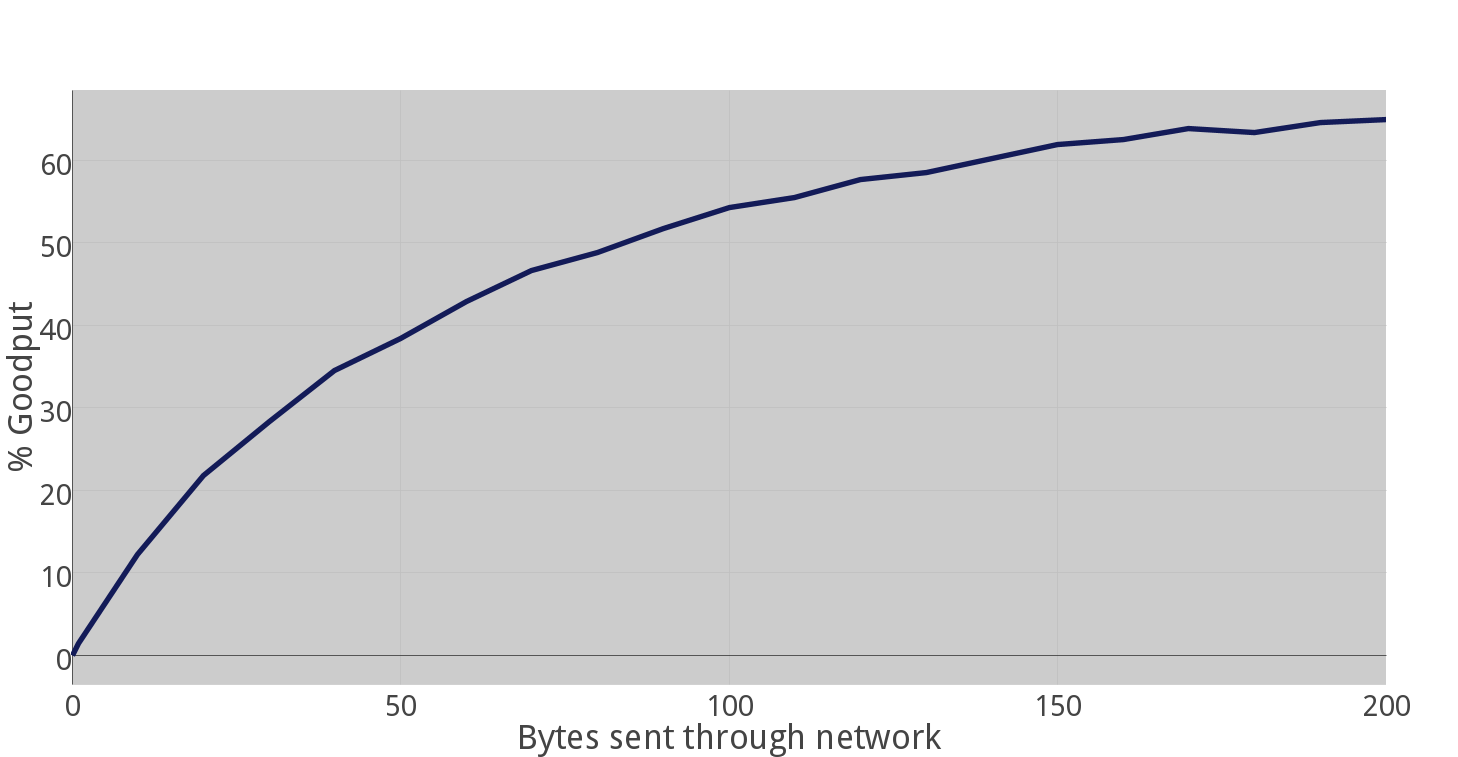
\includegraphics[scale=1.0]{NON0to200plotx09_thickerLineGRAY.png}    
%    \caption{NON 0-200 bytes }
%    \label{fig:NON0-200b}
%\end{figure}



% Removed after Davids read through
%\begin{figure}[ht]
%    \centering
%    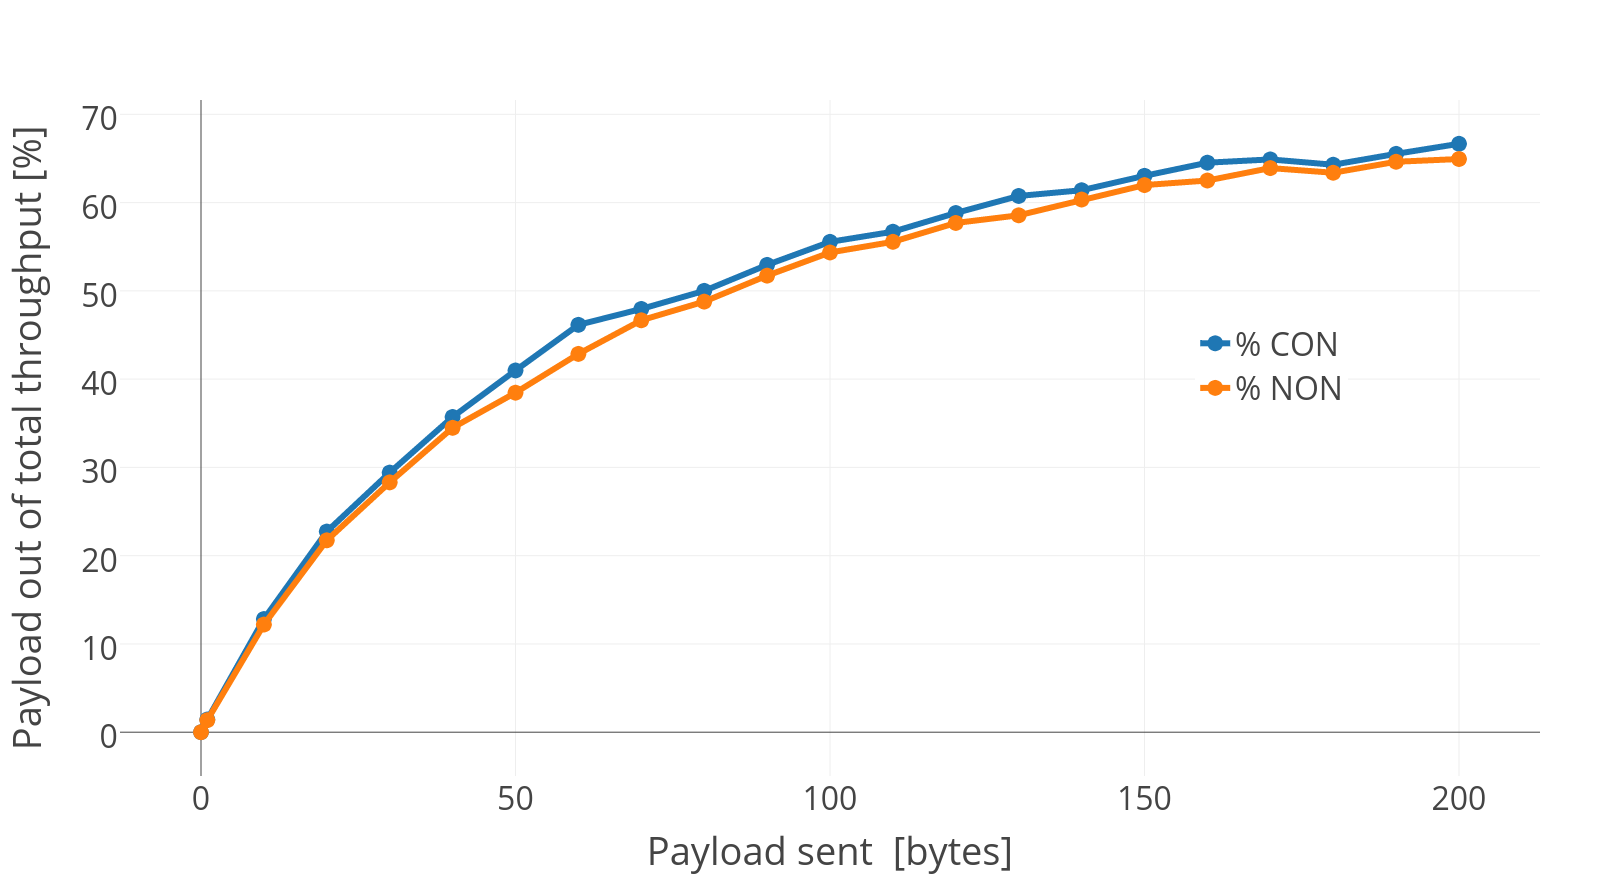
\includegraphics[width=1.0\textwidth]{CONvsNONplot_0-200_thicker3.png}    
%    \caption{CON vs NON 0-200 bytes}
%    \label{fig:CONvsNON0-200}
%\end{figure}

\begin{figure}[ht]
    \centering
    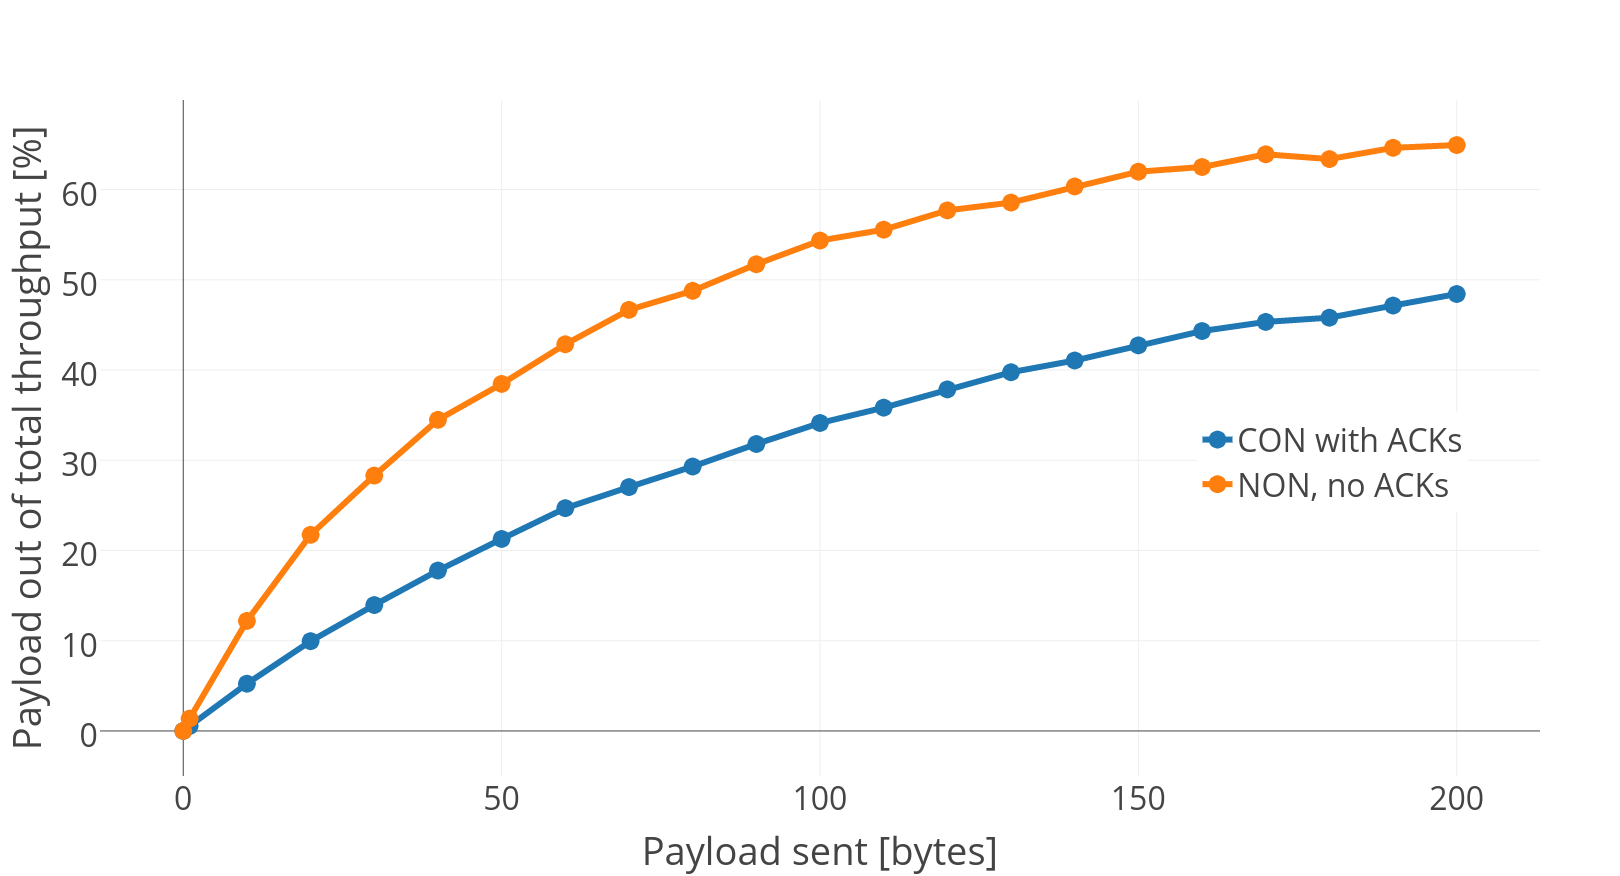
\includegraphics[width=1.0\textwidth]{CONNONvs0-200acks.png}    
    \caption{CON with ACKs vs NON 0-200 bytes}
    \label{fig:CONvsNON0-200_acks}
\end{figure}

\noindent Figure \ref{fig:CONvsNON0-200_acks} shows the comparison between sending between 0 and 200 bytes of useful data through the network. As expected from the Wireshark captures in the four previous tables, there are no major differences between these graphs when it comes to payload out of total throughput. The tables show that \gls{non} requires a few more bytes for each packet, which gives the difference between the two in this plot. 



\subsection{Discussion}

\noindent Even though these first tests were carried out with a very limited amount of data transferred, it is easy to see that the curves clearly flattens out and forms the shape of a \textit{parabola} with a vertical \textit{directrix} at \textit{x = 0}. Several \gls{ble} packets have been fragmented and sent during these test, without the graph showing a special \gls{payload} size where this gives a noticeable result. This means that the fragmentation of \gls{ble} packets does not have a major impact of the \% of payload compared to throughput in this system. More data needs to be sent at once to check if the same can be said for fragmentation of \gls{6lowpan} packets. The next step will be to transfer a larger amount of data, to verify that the assumptions that the graph will converge to the asymptotic value \textit{y = 87,1} when $lim_{x\to\infty}$. The limitations of transfer rate is not nearly yet met by neither \gls{ble} or \gls{6lowpan}.  These tests will therefore be explained in the next section. 

%\noindent There is already a clear trend in the form of the graph in figure \ref{fig:coapCON0200} even before the transfer rate reaches 200 bytes, but for small \glspl{payload} it is not very effective in these tests. If it is possible to find a way of transportation that could give a higher mathematical maximum, and also get to this limit faster, it could be very profitable to the system. It also makes sense to test \gls{coap} \gls{non} because it doesn’t need to send an \gls{ack} for every packet, as \gls{con} does. Maybe this means that the header files can be split up in another way, and that the useful amount of data sent through therefore will be higher. 


\noindent To see what happens when the limit of a \gls{6lowpan} packet was breached in the system, tests will be set up to send larger amounts of data than 200 bytes. The following test and examples will therefore send a fixed number of bytes at once from 0 to 1000 bytes (1 kB), with a 50 byte interval. This will also be a good way to test if the percentage of \gls{payload} compared to \gls{throughput} will converge to 87,1 \%, only considering \gls{ble} packets. As the previous tests, \gls{con} will transfer data using GET-messages, and therefore request a new message as soon as the \gls{ack} of the previous message has been received. \gls{non} has a fixed Max-Age value at 1 second, that determines the frequency of sending \gls{non} packets. 


\subsection{Tests with more data}

\noindent Table \ref{coapCON700table} shows a bigger and more complex case, where a payload of 700 byte is being sent at once using \gls{coap} \gls{con}. In total 889 bytes are being sent in this process, with a \gls{con} packet size of 774 bytes. This gives a percentage of \gls{payload} compared to \gls{throughput} at 78.74 \%. The maximum packet length of a \gls{6lowpan} packet at 127 bytes and the max in the testbed of 270 bytes are therefore exceeded. This can be seen in the table, after 8 \gls{ble} packages of 31 bytes each, have been sent, there is only room for 22 bytes in the last packet before the \gls{6lowpan} packet reaches its maximal capacity. This is repeated several times, once for each \gls{6lowpan} packet, until the last \gls{ble} packets at the size of 17 bytes. After this the standard packages for \gls{ack} and \textit{Number of completed packages} follows. This is a good example of how fragmentation of packets works in this system. 
%\todo{explain better, lower level 127, this system 270!} 


\begin{table}[H]
\small
\centering
\caption{Wireshark CoAP CON 700 bytes}
\label{coapCON700table}
\begin{tabular}{lllll}
\hline
Number & Time    & Protocol & Length & Info                             \\ \hline
%\rowcolor{blue} 
53     & 3.2570  & CoAP     & 774    & ACK, MID:35081, 2.05 Content     \\
%\rowcolor{38FFF8} 
54     & 3.2727  & CoAP     & 113    & CON, MID:35082, GET	              \\
55     & 3.4671  & HCI\_ACL & 31     & Rcvd {[}Reassembled in \#63{]}   \\
56     & 3.4747  & HCI\_ACL & 31     & Rcvd {[}Continuation to \#55{]}  \\
57     & 3.5374  & HCI\_ACL & 31     & Rcvd {[}Continuation to \#55{]}  \\
58     & 3.5375  & HCI\_ACL & 31     & Rcvd {[}Continuation to \#55{]}  \\
59     & 3.6077  & HCI\_ACL & 31     & Rcvd {[}Continuation to \#55{]}  \\
60     & 3.6078  & HCI\_ACL & 31     & Rcvd {[}Continuation to \#55{]}  \\
61     & 3.6767  & HCI\_ACL & 31     & Rcvd {[}Continuation to \#55{]}  \\
62     & 3.6782  & HCI\_ACL & 31     & Rcvd {[}Continuation to \#55{]}  \\
63     & 3.7533  & L2CAP    & 22     & Rcvd Connection oriented channel \\
64     & 3.7534  & L2CAP    & 16     & Sent LE Flow Control             \\
65     & 3.8172  & HCI\_EVT & 7      & Rcvd Number of Completed Packets \\
66     & 3.8172  & HCI\_ACL & 31     & Rcvd {[}Reassembled in \#74{]}   \\
67     & 3.8185  & HCI\_ACL & 31     & Rcvd {[}Continuation to \#66{]}  \\
68     & 3.9575  & HCI\_ACL & 31     & Rcvd {[}Continuation to \#66{]}  \\
69     & 3.9577  & HCI\_ACL & 31     & Rcvd {[}Continuation to \#66{]}  \\
70     & 4.0266  & HCI\_ACL & 31     & Rcvd {[}Continuation to \#66{]}  \\
71     & 4.0342  & HCI\_ACL & 31     & Rcvd {[}Continuation to \#66{]}  \\
72     & 4.0979  & HCI\_ACL & 31     & Rcvd {[}Continuation to \#66{]}  \\
73     & 4.0982  & HCI\_ACL & 31     & Rcvd {[}Continuation to \#66{]}  \\
74     & 4.1671  & L2CAP    & 22     & Rcvd Connection oriented channel \\
75     & 4.2372  & HCI\_ACL & 31     & Rcvd {[}Reassembled in \#83{]}   \\
76     & 4.2373  & HCI\_ACL & 31     & Rcvd {[}Continuation to \#75{]}  \\
77     & 4.3075  & HCI\_ACL & 31     & Rcvd {[}Continuation to \#75{]}  \\
78     & 4.3076  & HCI\_ACL & 31     & Rcvd {[}Continuation to \#75{]}  \\
79     & 4.3777  & HCI\_ACL & 31     & Rcvd {[}Continuation to \#75{]}  \\
80     & 4.4466  & HCI\_ACL & 31     & Rcvd {[}Continuation to \#75{]}  \\
81     & 4.4480  & HCI\_ACL & 31     & Rcvd {[}Continuation to \#75{]}  \\
82     & 4.4481  & HCI\_ACL & 31     & Rcvd {[}Continuation to \#75{]}  \\
83     & 4.5170  & L2CAP    & 22     & Rcvd Connection oriented channel \\
84     & 4.5871  & HCI\_ACK & 31     & Rcvd {[}Reassembled in \#86{]}   \\
85     & 4.5875  & HCI\_ACL & 31     & Rcvd {[}Continuation to \#84{]}  \\
86     & 4.6574  & L2CAP    & 17     & Rcvd Connection oriented channel \\
87     & 4.6731  & L2CAP    & 58     & Rcvd Connection oriented channel \\
88     & 4.6732  & L2CAP    & 50     & Rcvd Connection oriented channel \\
%\rowcolor[HTML]{38FFF8} 
89     & 4.6577  & CoAP     & 774    & ACK, MID:35082, 2.05 Content     \\
%\rowcolor[HTML]{38FFF8} 
90     & 4.6729  & CoAP     & 113    & CON, MID:35083, GET              \\ \hline
\end{tabular}
\end{table}

\newpage

\begin{table}[H]
\small
\centering
\caption{Wireshark CoAP NON 700 bytes}
\label{coapNON700table}
\begin{tabular}{lllll}
\hline
Number & Time    & Protocol & Length & Info                             \\ \hline
264    & 57.1476 & CoAP     & 777    & NON, MID:3, 2.05 Content         \\
265    & 57.2177 & HCI\_ACL & 31     & Rcvd {[}Reassembled in \#273{]}  \\
266    & 57.2178 & HCI\_ACL & 31     & Rcvd {[}Continuation to \#265{]} \\
267    & 57.2879 & HCI\_ACL & 31     & Rcvd {[}Continuation to \#265{]} \\
268    & 57.2943 & HCI\_ACL & 31     & Rcvd {[}Continuation to \#265{]} \\
269    & 57.3570 & HCI\_ACL & 31     & Rcvd {[}Continuation to \#265{]} \\
270    & 57.3583 & HCI\_ACL & 31     & Rcvd {[}Continuation to \#265{]} \\
271    & 57.4272 & HCI\_ACL & 31     & Rcvd {[}Continuation to \#265{]} \\
272    & 57.4286 & HCI\_ACL & 31     & Rcvd {[}Continuation to \#265{]} \\
273    & 57.4975 & L2CAP    & 22     & Rcvd Connection oriented channel \\
274    & 57.4979 & L2CAP    & 16     & Sent LE Flow Control             \\
275    & 57.5676 & HCI\_ACL & 31     & Rcvd {[}Reassembled in \#284{]}  \\
276    & 57.5685 & HCI\_EVT & 7      & Rcvd Number of Completed Packets \\
277    & 57.5753 & HCI\_ACL & 31     & Rcvd {[}Continuation to \#275{]} \\
278    & 57.6378 & HCI\_ACL & 31     & Rcvd {[}Continuation to \#275{]} \\
279    & 57.6379 & HCI\_ACL & 31     & Rcvd {[}Continuation to \#275{]} \\
279    & 57.7080 & HCI\_ACL & 31     & Rcvd {[}Continuation to \#275{]} \\
280    & 57.7082 & HCI\_ACL & 31     & Rcvd {[}Continuation to \#275{]} \\
281    & 57.7771 & HCI\_ACL & 31     & Rcvd {[}Continuation to \#275{]} \\
282    & 57.7785 & HCI\_ACL & 31     & Rcvd {[}Continuation to \#275{]} \\
283    & 57.7785 & HCI\_ACL & 31     & Rcvd {[}Continuation to \#275{]} \\
284    & 57.8474 & L2CAP    & 22     & Rcvd Connection oriented channel \\
285    & 57.9176 & HCI\_ACL & 31     & Rcvd {[}Reassembled in \#293{]}  \\
286    & 57.9176 & HCI\_ACL & 31     & Rcvd {[}Continuation to \#285{]} \\
287    & 57.9878 & HCI\_ACL & 31     & Rcvd {[}Continuation to \#285{]} \\
288    & 57.9879 & HCI\_ACL & 31     & Rcvd {[}Continuation to \#285{]} \\
289    & 58.0580 & HCI\_ACL & 31     & Rcvd {[}Continuation to \#285{]} \\
290    & 58.0581 & HCI\_ACL & 31     & Rcvd {[}Continuation to \#285{]} \\
291    & 58.1270 & HCI\_ACL & 31     & Rcvd {[}Continuation to \#285{]} \\
292    & 58.1284 & HCI\_ACL & 31     & Rcvd {[}Continuation to \#285{]} \\
293    & 58.1972 & L2CAP    & 22     & Rcvd Connection oriented channel \\
294    & 58.2673 & HCI\_ACK & 31     & Rcvd {[}Reassembled in \#296{]}  \\
295    & 58.2688 & HCI\_ACL & 31     & Rcvd {[}Continuation to \#294{]} \\
296    & 58.3378 & L2CAP    & 20     & Rcvd Connection oriented channel \\
297    & 58.3379 & CoAP     & 777    & NON, MID:4, 2.05 Content         \\ \hline
\end{tabular}
\end{table}

\noindent Table \ref{coapCON700table} shows a bigger and more complex case, where a payload of 700 byte is being sent at once using \gls{coap} \gls{con}. In total 889 bytes are being sent in this process, which consists of four \gls{6lowpan} packets where three of them is the full 270 bytes. This can be seen in the table, after 8 \gls{ble} packages of 31 bytes each has been sent, there is only room for 22 bytes in the last packet before the \gls{6lowpan} packet has reached its maximal capacity. The last packet contains $31+31+17 = 79 \, bytes$, which leaves 199 unexploited bytes in the packet. Concerning fragmentation, it would probably have been better to send data with a slightly smaller payload. After this the standard packages for \gls{ack} and \textit{Number of completed packages} follows. This is a good example of how fragmentation of packets works in this system.  The percentage of \gls{payload} compared to \gls{throughput} is therefore 700 bytes/889 bytes = 78,74 \% in this case. 

\noindent As a direct comparison, table \ref{coapNON700table} represents the same \gls{goodput} sent through the network using \gls{coap} \gls{non}. In this case, the total is 892 bytes, only three more than the previous example. This confirms that \gls{con} and \gls{non} works in very similar ways when it comes to packet fragmentation, and the same pattern of 270 bytes \gls{6lowpan} packets is being recognised. Calculations shows that in this case the percentage is 700 bytes/892 bytes = 78,47 \%. 

%\ Sendt 912 pakker..??!?!?!?

%\begin{figure}[ht]
%    \centering
%    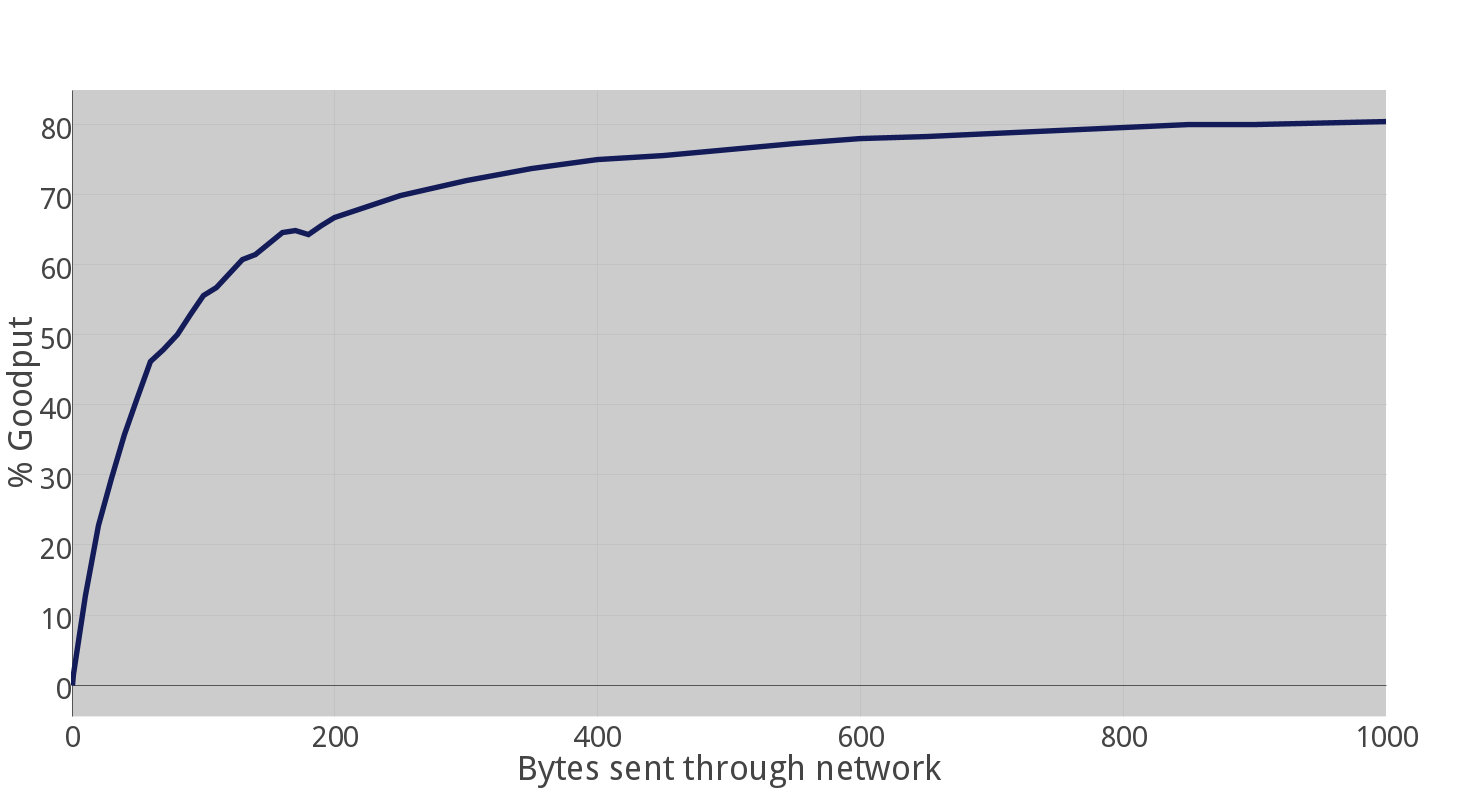
\includegraphics[width=\textwidth]{CON0toK_thickerGRAY.png}    
%    \caption{CoAP CON plot, 200 bytes to 1 kB}
%    \label{fig:plotCoAPCON200toK}
%\end{figure}

\subsection{Discussion}

\noindent Using these results from measurements of \glspl{payload} between 0 and 1000 bytes it was possible to plot the graph in figure \ref{fig:NON0-kb}. Here it is easy to see the same trends as in figure \ref{fig:coapCON0200}, but over a wider span of sent bytes. These results are as expected after the previous tests, and in compliance with the calculations done concerning horizontal asymptote.  

%\begin{figure}[ht]
%    \centering
%    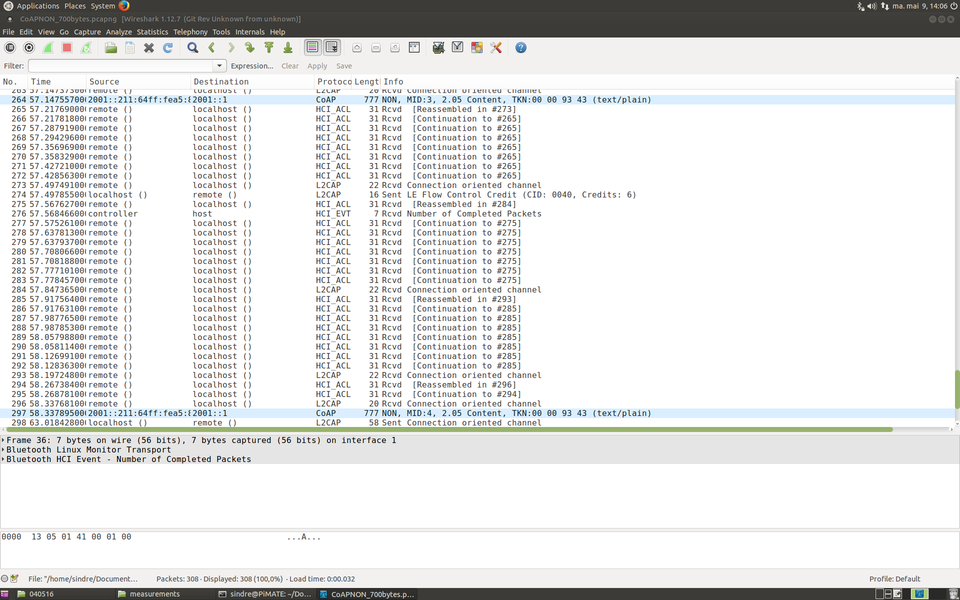
\includegraphics[scale=0.40]{rsz_1coapnon_wireshark700fullscreen.png}    
%    \caption{CoAP NON 700 bytes Wireshark capture}
%    \label{fig:NON7000bytesFullWireshark}
%\end{figure}

\noindent Table \ref{coapCON700table} and \ref{coapNON700table} shows the case where 700 bytes where sent at once through the network, using both \gls{coap} \gls{con} and \gls{non}. The size of fragmented packet was very similar in both cases and the percentage of \gls{payload} compared to \gls{throughput}, but \gls{con} needs \glspl{ack} in addition. 

\begin{equation} \label{lessThanHAlfAPercentCalculation}
	\frac{700 \, bytes \, payload}{889 \, bytes \, throughput \, + \, 113 \, bytes \, ack} = 69,86 \,\%
\end{equation}
\begin{equation} \label{lessThanHAlfAPercentCalculation2}
	\frac{700 \, bytes \, payload}{892 \, bytes \, throughput} = 78,48 \,\%
\end{equation}	
\begin{equation} \label{lessThanHAlfAPercentCalculation3}	
    \frac{69,86}{78,48} \approx 0,8902  \rightarrow 100 \% - 89,02 \% = 10,98 \,\%
\end{equation}
%\todo{Explain equation better}

\noindent Calculations in equation \ref{lessThanHAlfAPercentCalculation} show that the percentage of \gls{payload} \gls{con} is 78,48 \%, compared to 69,86 \% in \gls{con}. The difference between these two is \textit{10,98 \%}. This can also be seen clearly in \ref{fig:NON0-kb2}. Because of this, it was concluded that the results for using \gls{non} and \gls{con} can be considered as negligible for transmissions larger than 1 kB. Tests with larger amounts of data than this at once did therefore not seem necessary, and will not be investigated in this project. 

% Removed after David read through
%\begin{figure}[ht]
%    \centering
%    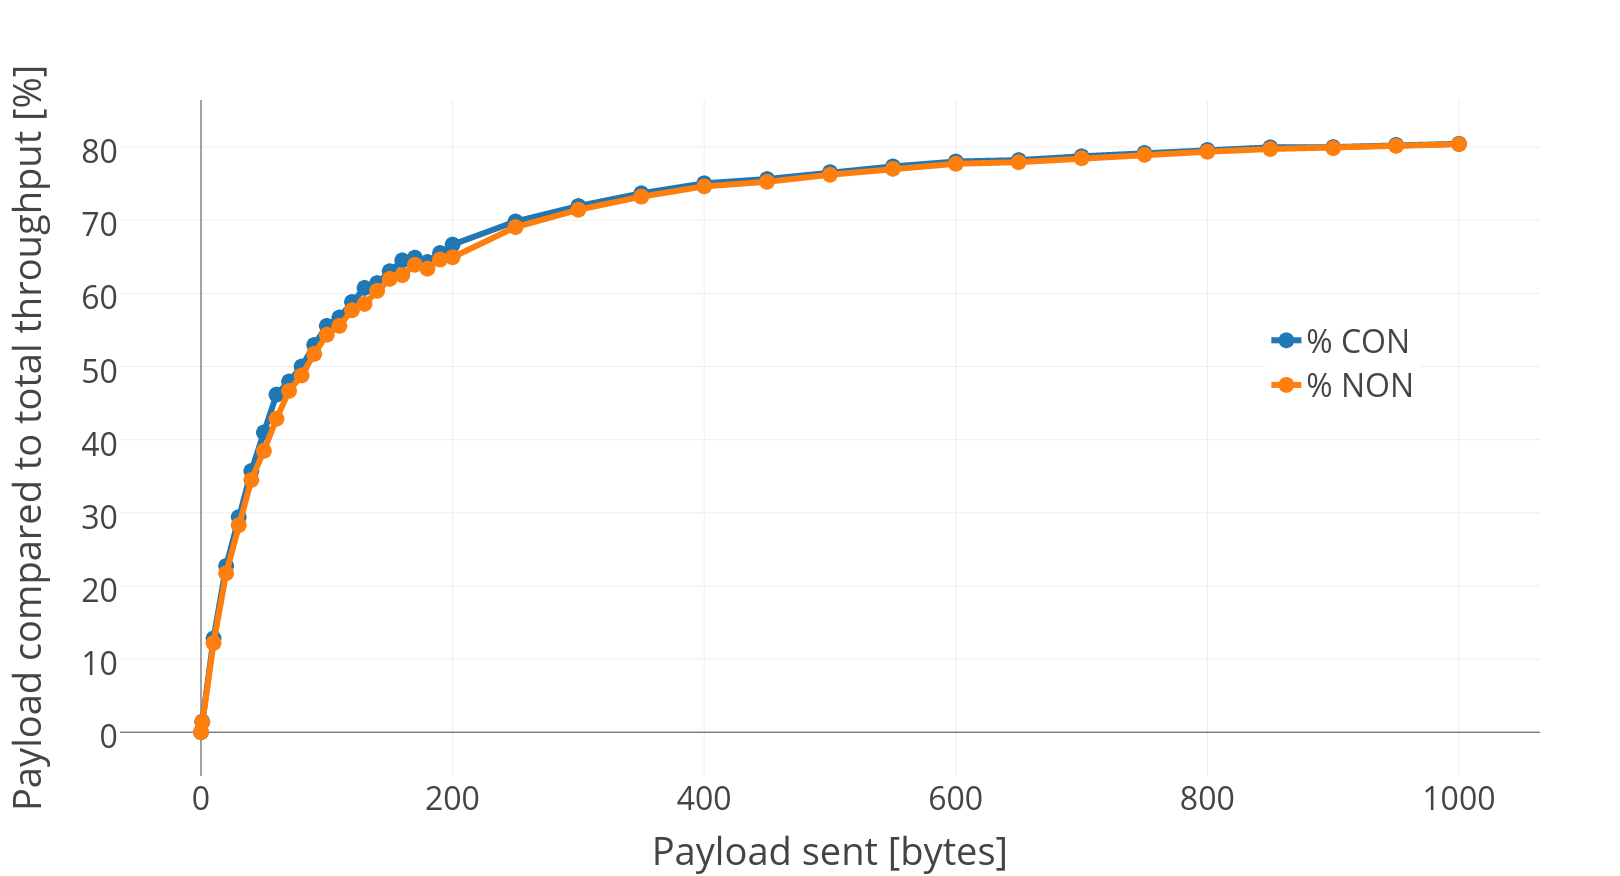
\includegraphics[width=1.0\textwidth]{CONvsNON0tokilobytes.png}    
%    \caption{CON vs NON 0-1000 bytes}
%    \label{fig:NON0-kb}
%\end{figure}


\begin{figure}[ht]
    \centering
    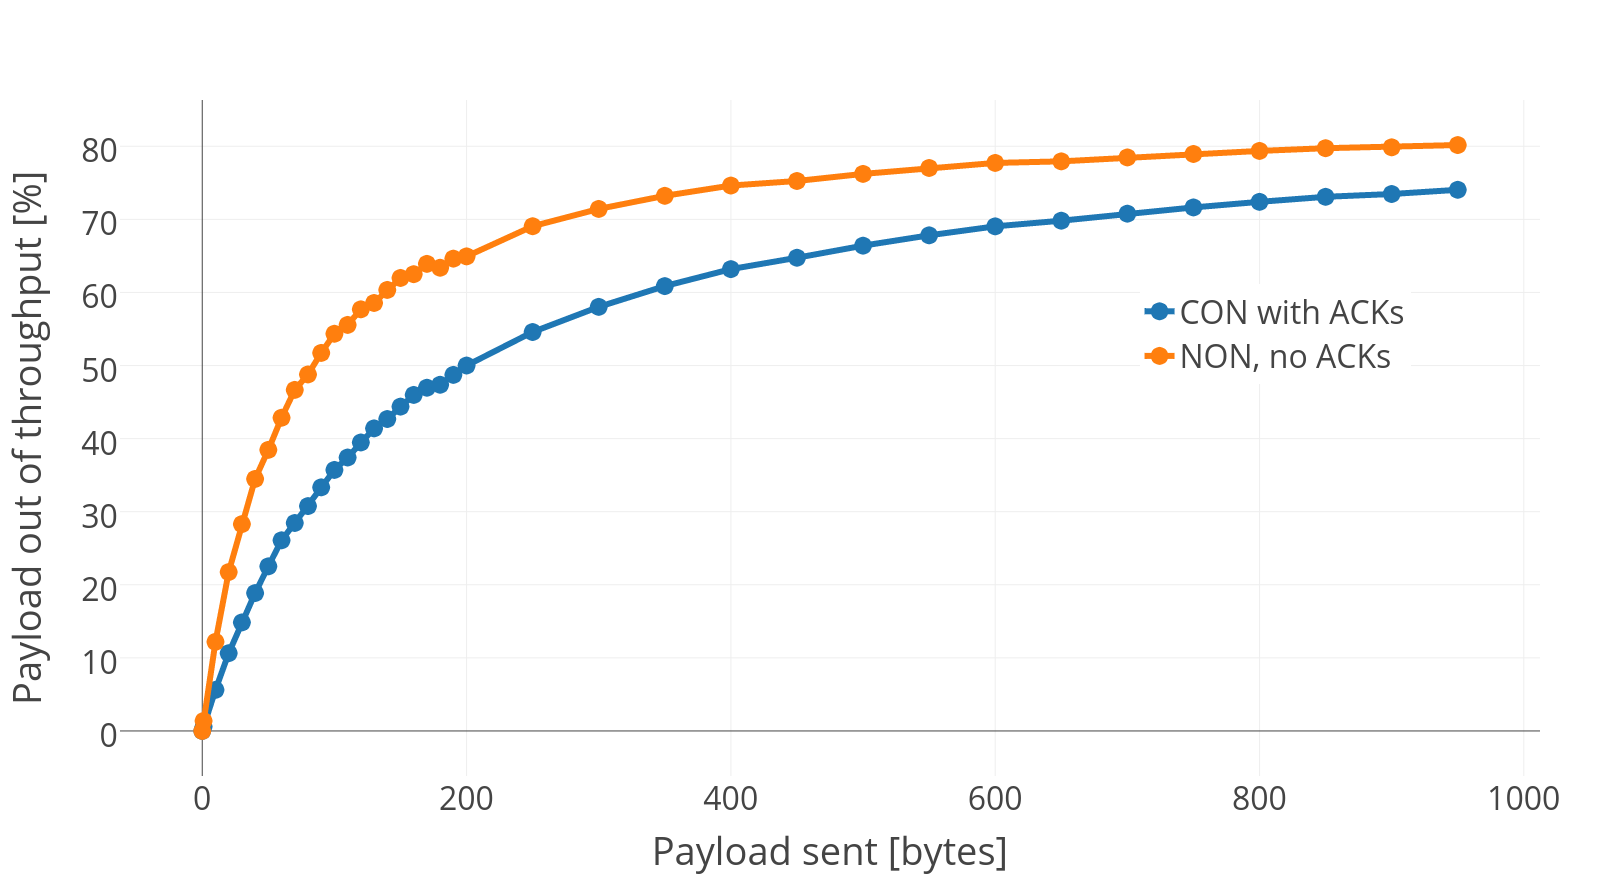
\includegraphics[width=1.0\textwidth]{CONNON0-kwithACK.png}    
    \caption{CON with ACKs vs NON 0-1000 bytes}
    \label{fig:NON0-kb2}
\end{figure}


\noindent Given these results, it can be concluded that to send less data than 200 bytes at the time is not preferable, since the percentage of \gls{payload} compared to the total amount sent can be very low. On the other hand, the graph stabilizes around 65-70 \% for \gls{con} and 75-80 \% for \gls{non}. Given these measurements it looks like 400 bytes and bigger packets are preferable in this system. The system shows no signs of weakness as the packet size grows, and it will therefore in theory be possible to send as large packets as needed until the limitations of \gls{ble} with the same amount of goodput at about 80 \%. This was however never achieved in this configuration of the network, but should be possible to do in future works. Concerning fragmentation, it was concluded after having sent \glspl{payload} up to 200 bytes that fragmentation of \gls{ble} packets is not a major concern in this network. After having sent up to 1000 bytes to check the same for \gls{6lowpan} packets, the same thing can be concluded here. Both graphs of \gls{con} and \gls{non} shown in \ref{fig:NON0-kb2} show a flat and stable curve, with no special weak points in the different \glspl{payload}. This would be expected right after the \gls{payload} was big enough to exceed a \gls{ble} or \gls{6lowpan} packet, just as explained in chapter \ref{chp:measurements2}.2.2. Developers should therefore not consider to minimize the \gls{payload} just to avoid fragmentation, in such a network. 




\section{Transfer rates}

\subsection{Time used to transfer payload}

\noindent Previous sections in this chapter have shown the percentage of payload compared to the total throughput, to measure if fragmentation was a major concern in this network. This is a good overview of how the protocols are able to exploit the network, and tells a lot about the different protocols. Developers could possibly use these results to build the \gls{iot} network. For end users in a real world scenario however, the actual \textit{throughput per time} would be more relevant, since this tells how much data can be transported every second. A common measuring unit for this is known as \textit{\gls{goodput}}, measured in bytes per second.  



\noindent There are several ways to measure throughput compared to time used. For instance by calculating the number of seconds it takes to transfer a known number of bytes, or the number of bytes that are transported on average every second. To calculate this, values from measurements shown in table \ref{goodputTimeCON} and \ref{goodputTimeNON} in appendix \ref{chp:appendixb} were used. The numbers shown in these tables and used in the following experiments have been measured by sending a considerable amount of packets through the network\footnote{All measurements can be seen on GitHub: \url{https://github.com/sische/MasterThesis}}. In most cases more than 100 \gls{coap} packets was sent for each constant payload, to find the minimum, average and maximum value for both the time used to transfer a packet and the \gls{goodput} in each case. 
%The rest of the experiment is well documented data, based on measured values which can be found on \url{https://github.com/sische/MasterThesis/measurements}.  

\begin{figure}[h!]
    \centering
    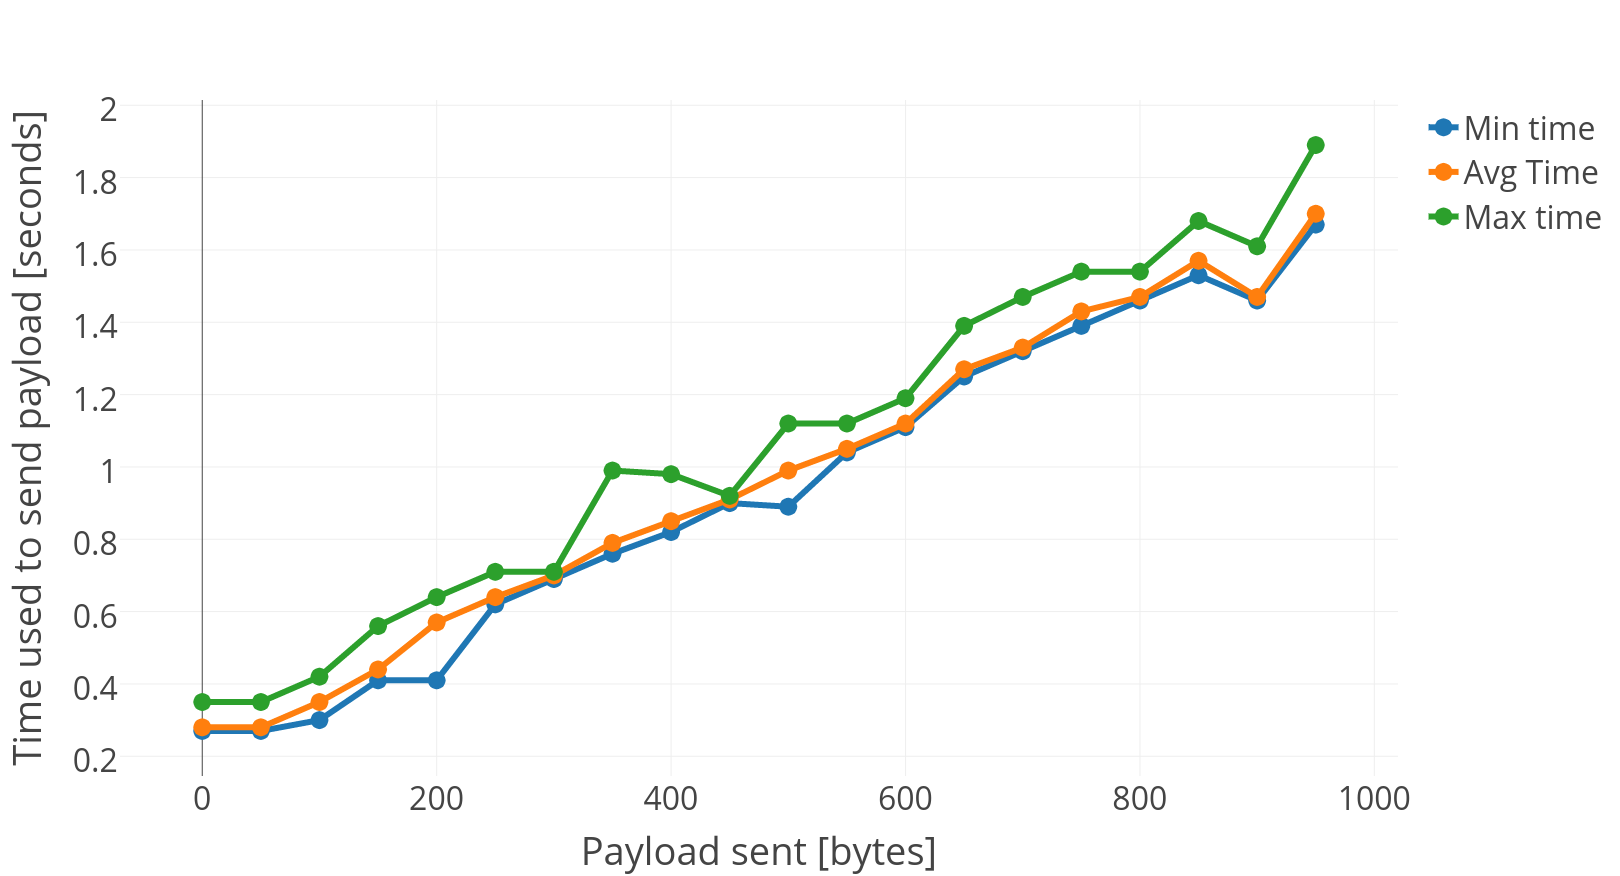
\includegraphics[width=1.0\textwidth]{bytesPrSecondNew3.png}    
    \caption{Time used to transfer payload CON}
    \label{fig:bytesPRSecond3}
\end{figure}


\noindent Figure \ref{fig:bytesPRSecond3} shows the minimum, average and maximum time it took to send a constant payload through the network using \gls{con}. This variation is relevant to see the stability in the network, how much it can be trusted. A system carrying important data needs a stable transfer rate at all times, not only a good average value. In this case the largest deviation from the average value is at 350 bytes, where the max. value is almost 1 second, while the average is approximately 0.7 seconds. Both the average and minimum graph has a quite linear development, with the exception of 900 bytes. The lowest transfer rate for \gls{con} is when the payload is below 100 bytes. The transfer time at this payload is about 300 \textit{ms}, which seems logical concerning the ping tests in the beginning of the chapter at 250 \textit{ms}. The slowest transfer time is the max value when transferring 950 bytes, when the time is approaching 2 seconds.  


\begin{figure}[h!]
    \centering
    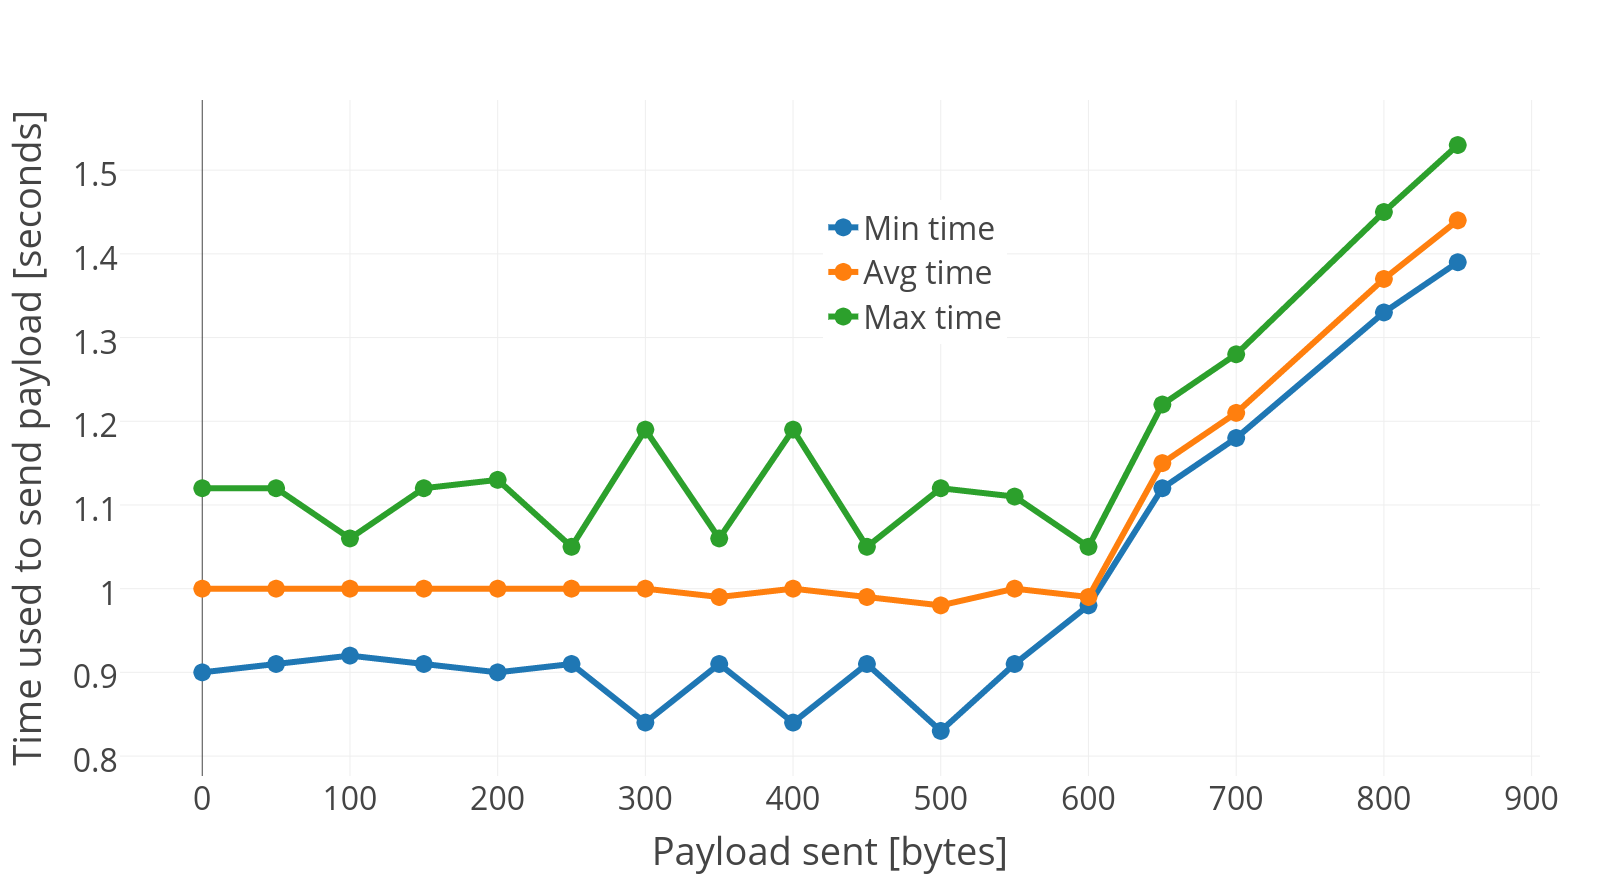
\includegraphics[width=1.0\textwidth]{bytesPrSecondNewNON.png}    
    \caption{Time used to transfer payload NON}
    \label{fig:bytesPRSecond4}
\end{figure}

\noindent Time used to transfer a given payload using \gls{non} can be seen in figure \ref{fig:bytesPRSecond4}. Even thought there are some slight variations from min. to max. time used, the average transfer frequency is very stable. Because of the described difficulties concerning Max-Age of the measured field in \gls{non}, the fastest transfer frequency achieved in the system was 1 second. On average the transfer rate is very close to this, but the min and max values vary from 0.85 seconds to 1.2 seconds in both 300 and 400 bytes payload. 600 bytes is the maximum payload where the system is still able to transfer data at 1 second rate, after this the graph starts to climb for larger payloads. For \gls{non} with a payload larger than 650 bytes, the network was too unstable to do the same amount of data as in previous tests. These values (NON > 650 bytes payload) are therefore not as certain as the rest of the tests considering amount of packets sent.


\begin{figure}[h!]
    \centering
    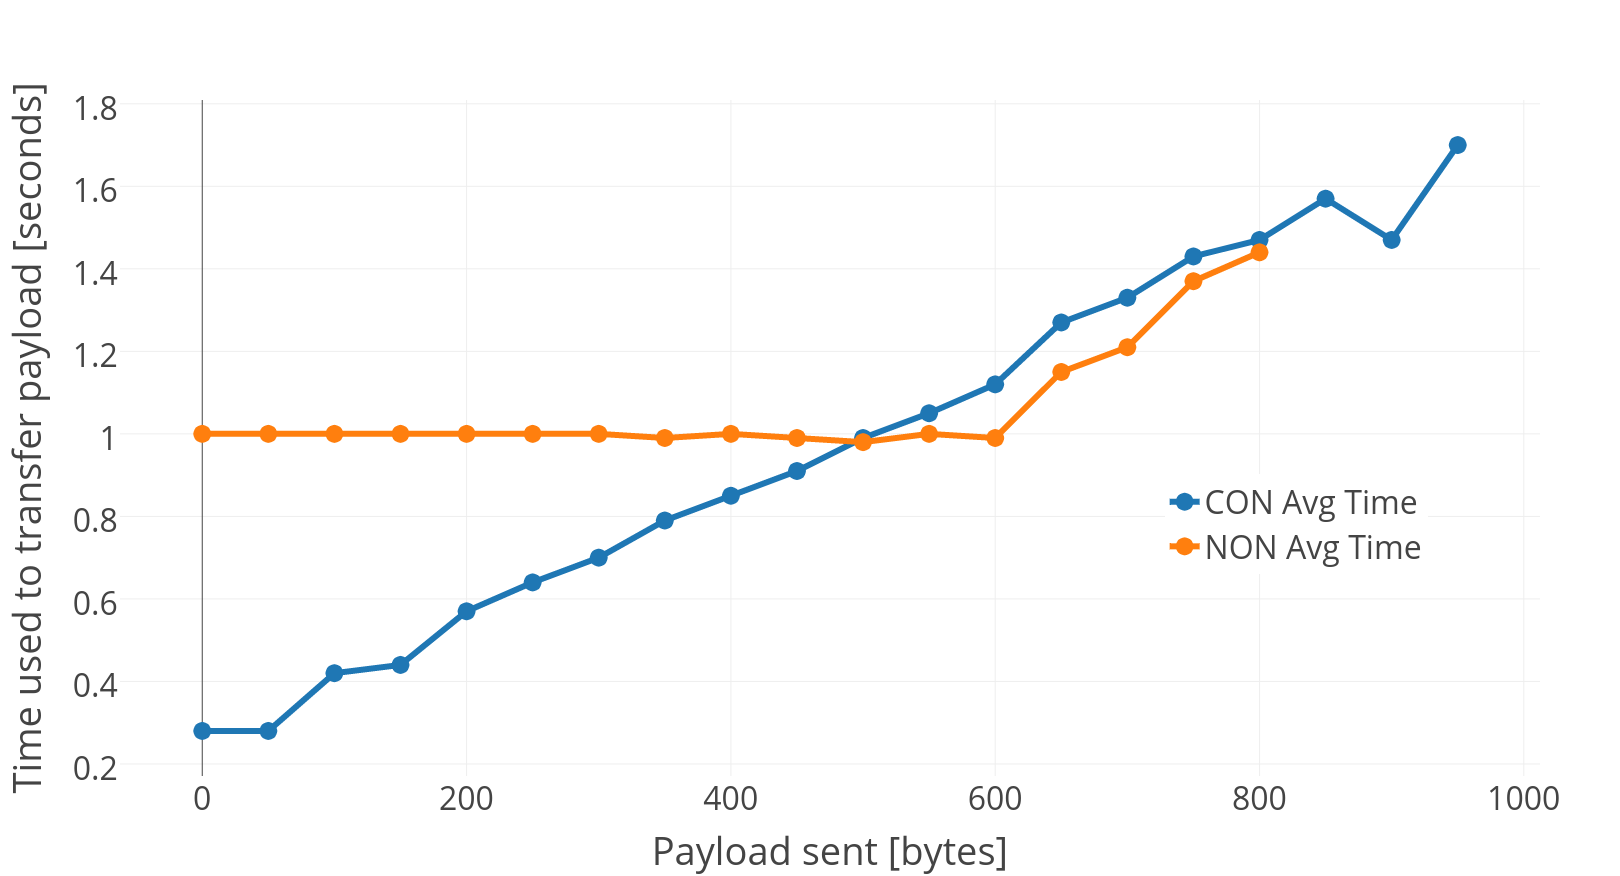
\includegraphics[width=1.0\textwidth]{avgTimeCONNON.png}    
    \caption{Average time to transfer payload, CON vs NON}
    \label{fig:avgTimeCONNON}
\end{figure}




%\begin{figure}[h!]
%    \centering
%    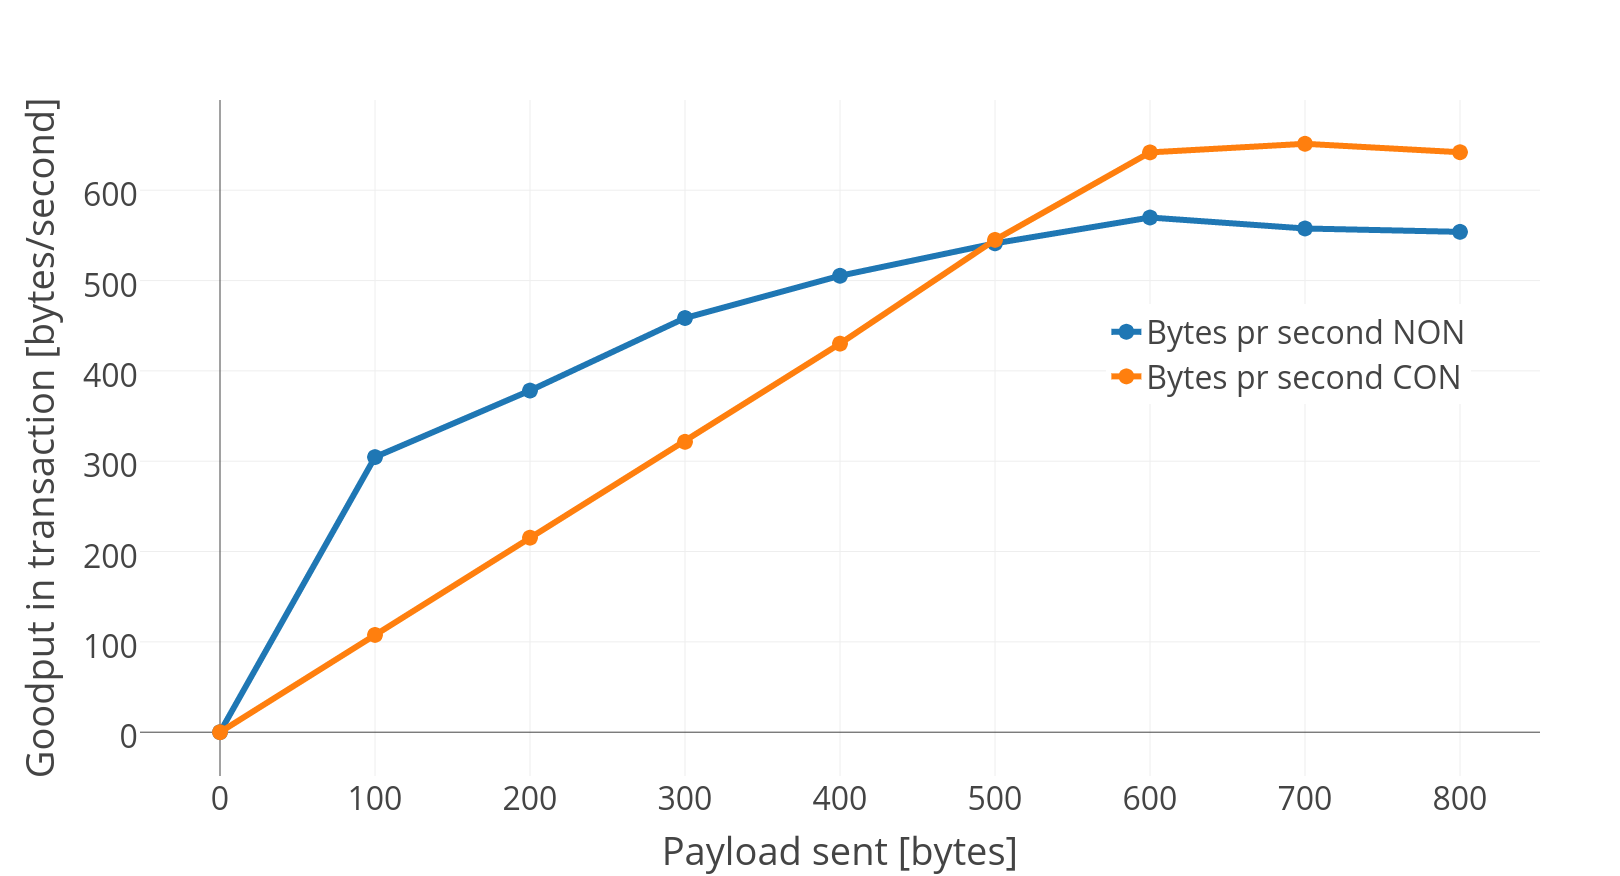
\includegraphics[width=1.0\textwidth]{bytesPRSecond3.png}    
%    \caption{Number of bytes per second}
%    \label{fig:bytesPRSecond2}
%\end{figure}

\noindent To get a direct comparison of these data, the average values from \gls{con} and \gls{non} are being compared in figure \ref{fig:avgTimeCONNON}. This makes the differences between the two easy to spot. It takes 0.4 \textit{seconds} to transfer 100 bytes \gls{goodput} in \gls{con}, while it takes 1 \textit{second} using \gls{non}. However, as the graph shows, if the goodput is 500 byte, both versions of the protocol uses \textit{1} second to transfer the data. When the \gls{payload} reaches 600 byte, \gls{con} needs to use 1,15 \textit{seconds} to transfer the data, while \gls{non} is still able to only use \textit{1} second. After this \gls{con} is about 150 \textit{ms} slower than \textit{non} to transfer the same payload, but this gap closes as the payload gets higher. In this case it is quite easy to see a trend -- \gls{con} is definitely faster at small rates of data, below 500 byte. If the payload is bigger than this, \gls{non} will be preferable, only taking the time to transfer a given number of data one way into account.

%\subsection{Discussion}

%Previous graphical figures shows  
%\todo{Write in end-discussion}


%\subsection{Goodput}

\noindent From another approach, it is possible to look at how many bytes can be sent for every given time using the two different versions of the protocol. This is profitable because it will show which payload size that gives the maximal \gls{throughput} for every time interval, and can possibly be exploited by both a developer and an end user in such a system. Figure \ref{fig:goodPayload_CON} shows the direct correlation between the number of bytes sent every second. 

\begin{figure}[ht]
    \centering
    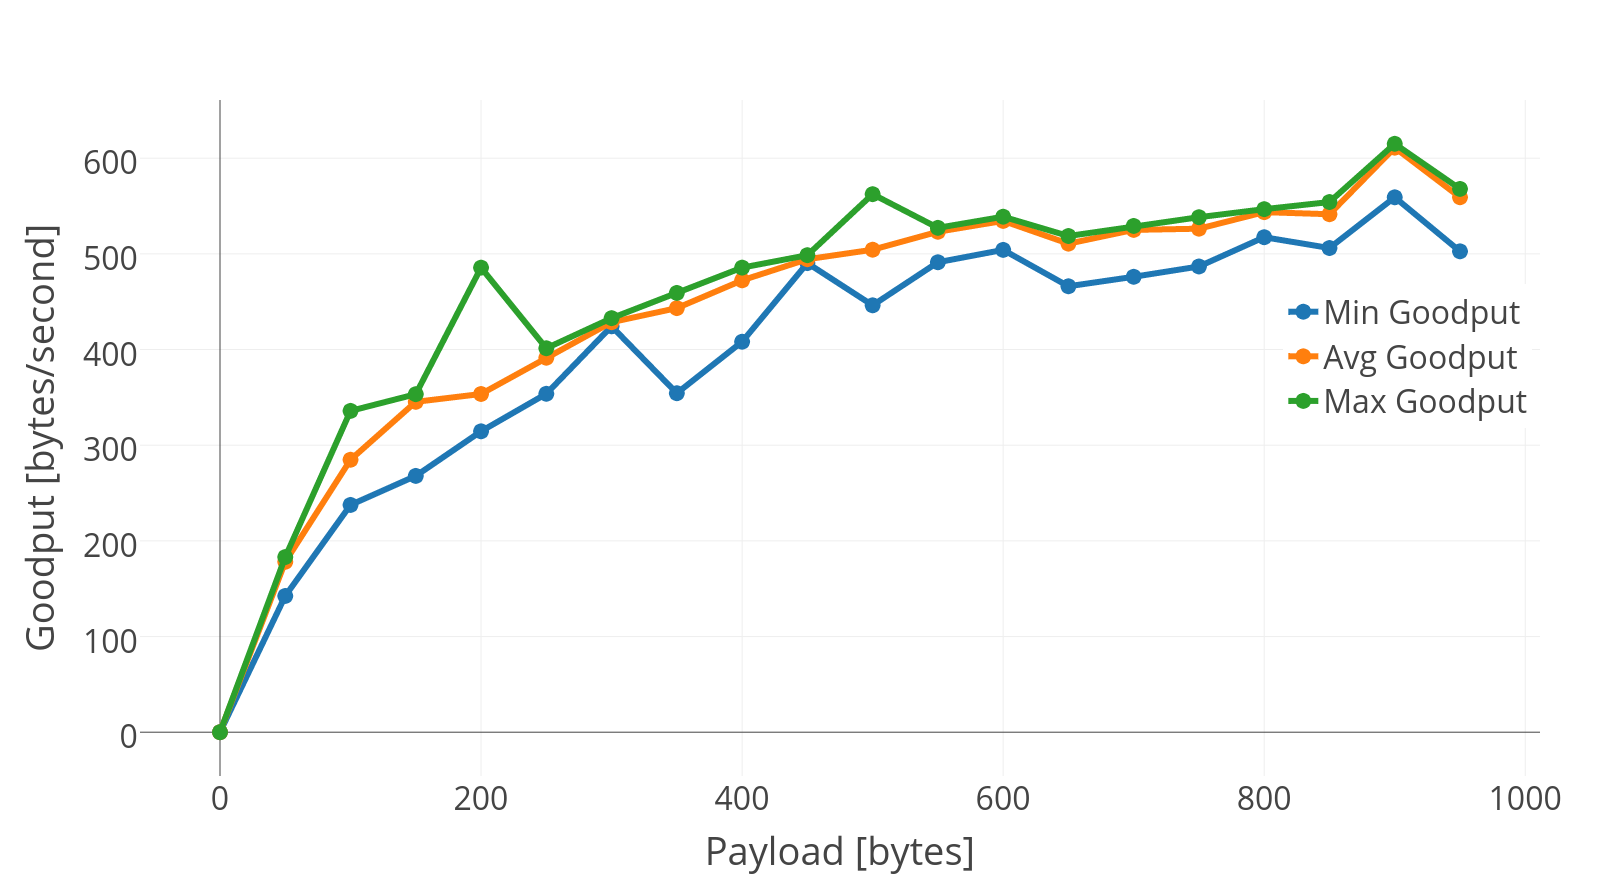
\includegraphics[width=1.0\textwidth]{goodput_payload_CON.png}    
    \caption{Goodput compared to payload CoAP CON}
    \label{fig:goodPayload_CON}
\end{figure}

\begin{figure}[h!]
    \centering
    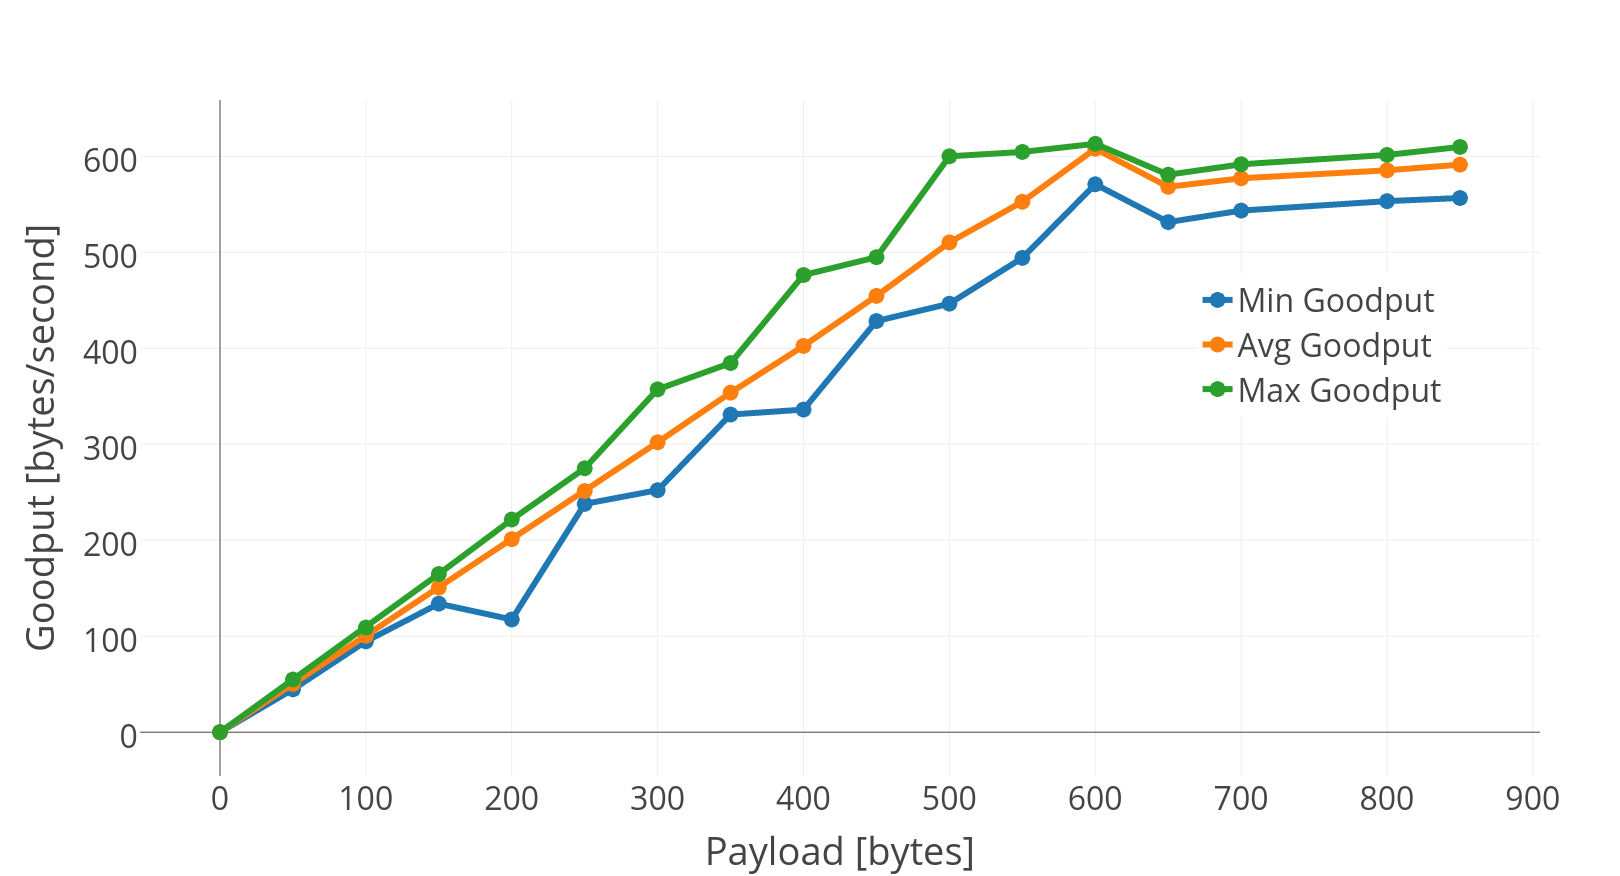
\includegraphics[width=1.0\textwidth]{goodput_payload_NON.png}    
    \caption{Goodput compared to payload CoAP NON}
    \label{fig:goodPayload_NON}
\end{figure}


\noindent As in the previous tests, it is preferable to have a stable \gls{goodput} through the network, to be able to calculate and predict the capacity of the network. Figure \ref{fig:goodPayload_CON} shows the minimum, average and maximum values of \gls{goodput} using \gls{con}. The values are in general quite stable, with a few exceptions of the min and max values measured probably caused by disturbance in the network. The graph rises fast at low payload, and later flattens out. The highest achieved \gls{goodput} in these tests was 611 bytes/second when the \gls{payload} was 900 bytes. It reached 500 bytes/second at 500 bytes \gls{payload}. From this graph it looks like the maximum transfer rate using \gls{con} is approximately 700 bytes, and will probably never hit 1 kB per second. 

\noindent In the same case using \gls{non}, the graph starts to climb almost linear with a climbing rate of 100 bytes/second added for every 100 byte payload added, as seen in figure \ref{fig:goodPayload_NON}. This makes sense, given that the transfer interval is constant at once per second for \gls{payload} sizes from 0 to 600 bytes. Variation to min and max values occurs, but not more than expected compared to previous results. The highest achieved \gls{goodput} is 608 bytes/second, almost exactly the same as the maximum achieved in \gls{con}. For \glspl{payload} higher than this the \gls{goodput} drops down to about 580 and stays more or less constant there \footnote{Keep in mind that measurements for payload > 650 bytes in NON are unstable links, and does not rely on the same number of measurements as the rest of the tests}.


\noindent The direct comparison of the average values of \gls{goodput} using \gls{con} and \gls{non} can be seen in figure \ref{fig:payloadGoodput_CONNON}. In this case both plots starts at 0 bytes/second, since the payload is 0. After this, the graphs have quite different forms. \gls{non} has a very linear rise, all the way up to 600 byte payload. When transferring a payload of 100 bytes, \gls{con} is almost three times faster at \textit{305 bytes/second} compared to \textit{108 byte/second} using \gls{non}. \gls{con} therefore looks significantly more efficient for a small amount of data, but for payload bigger than 500 byte \gls{non} is preferable in this system.

\begin{figure}[ht]
    \centering
    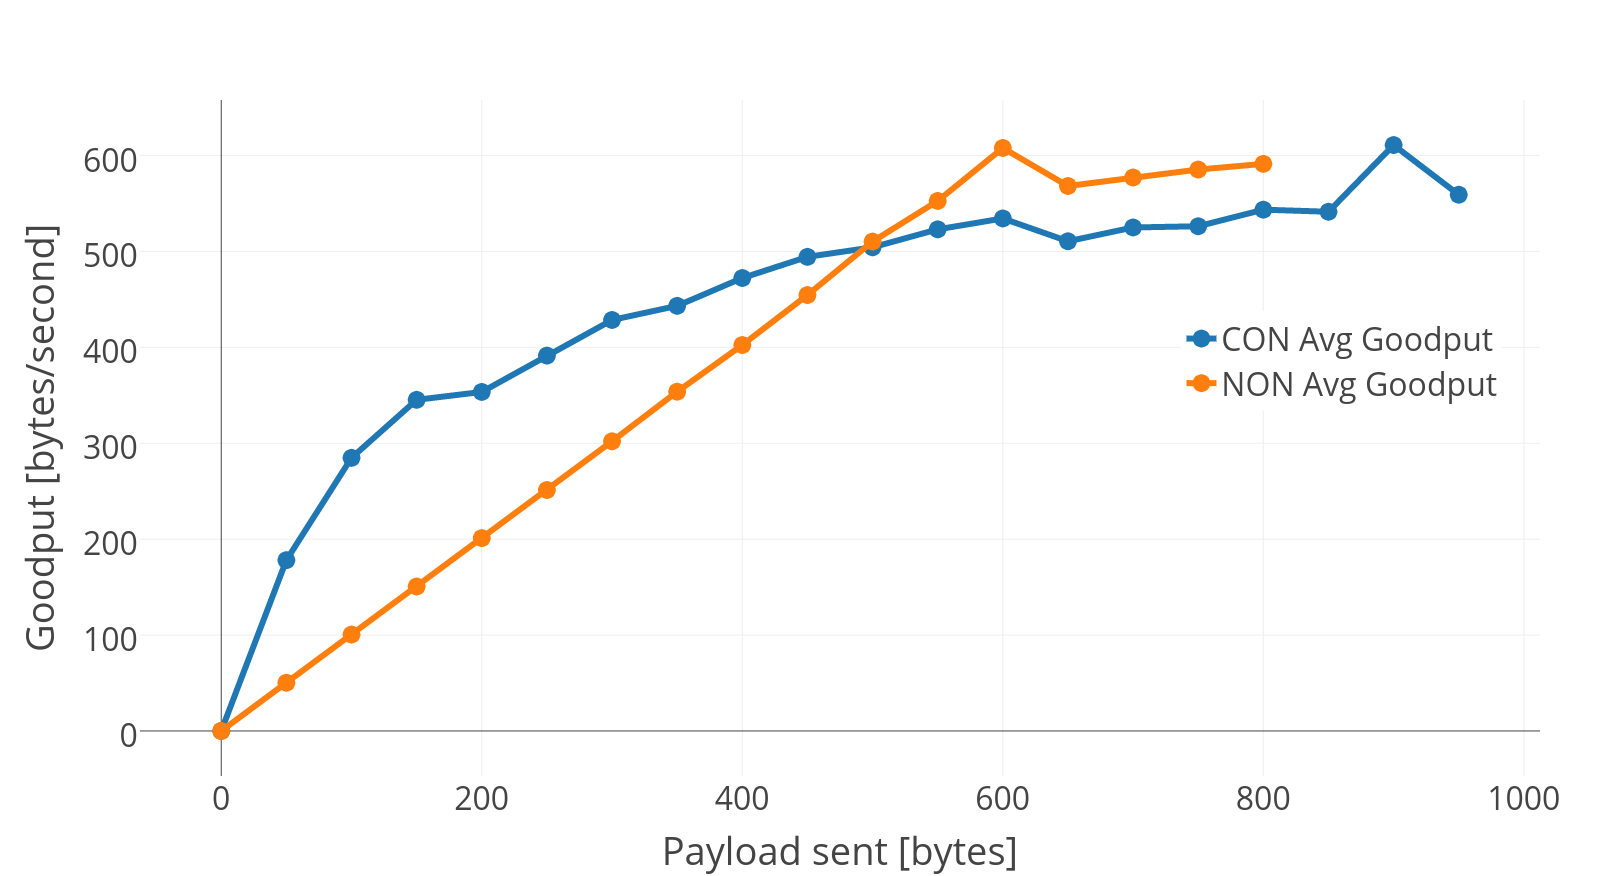
\includegraphics[width=1.0\textwidth]{payloadGoodput_CONNON.png}    
    \caption{Goodput for given payload, CON vs NON}
    \label{fig:payloadGoodput_CONNON}
\end{figure}
 


%\begin{figure}[ht]
%    \centering
%    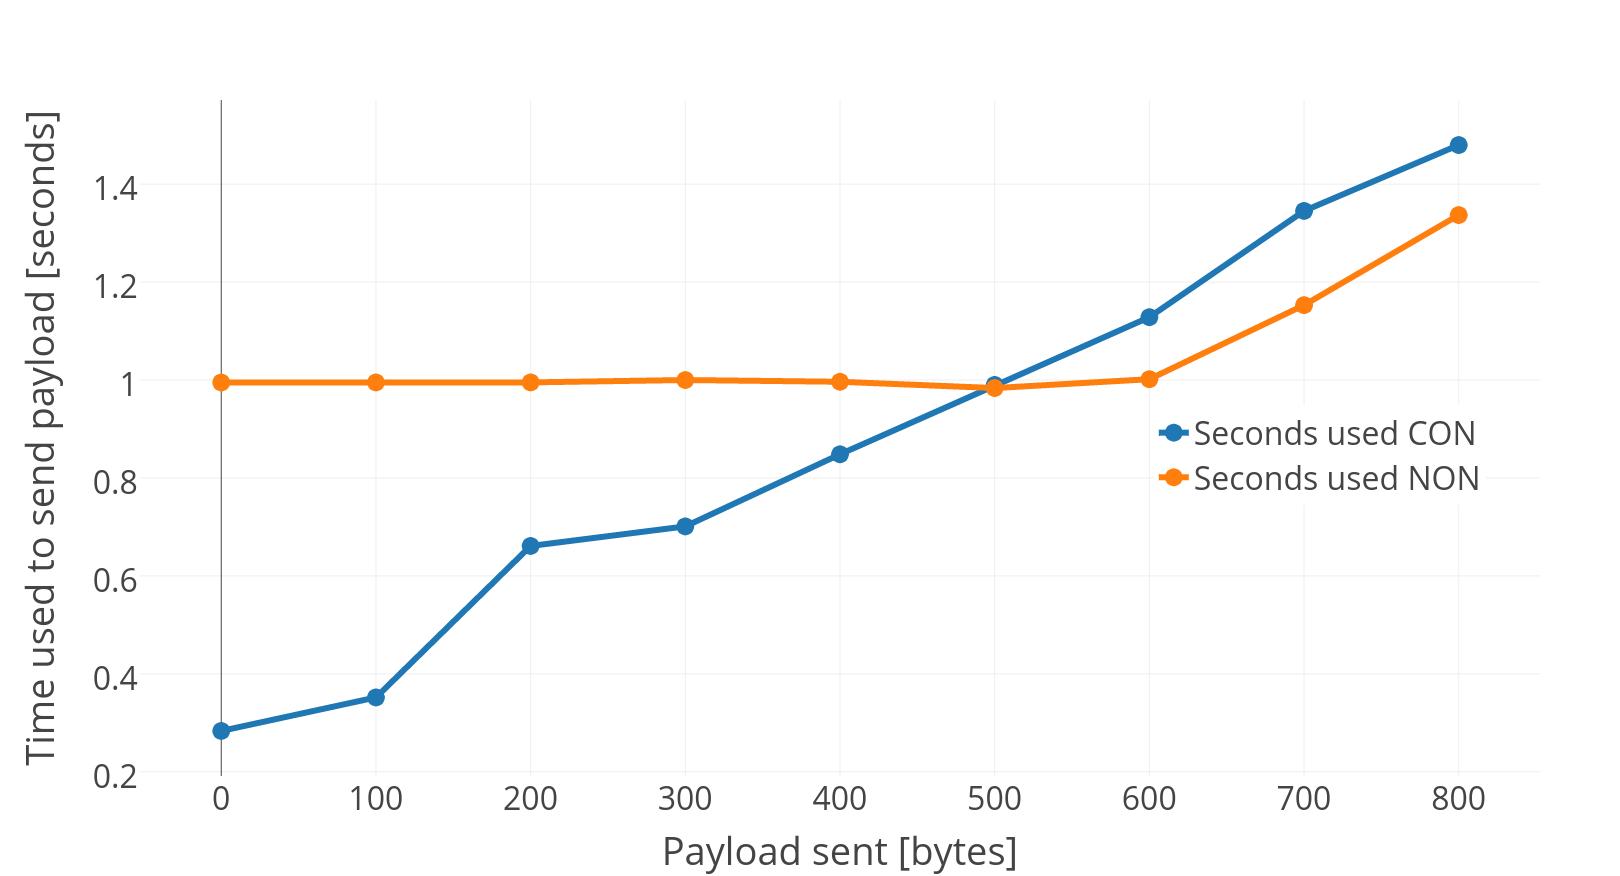
\includegraphics[width=1.0\textwidth]{timeUsedPRpacket3.png}    
%    \caption{Time used per packet, OLD}
%    \label{fig:timeUsedPRpacket}
%\end{figure}

\newpage
\subsection{Bytes sent through network, best and worst case}

\noindent These previous two tests shows the throughput per time, while the tests earlier in the thesis has focused on the amount of throughput that is \gls{payload}, how much of the data sent is useful data. Since these \glspl{microcontroller} are used as end nodes in the network, it is natural to assume that they will run on battery power only. In this case it is preferable that they do as little work as possible, meaning also handle as few packets as possible. It will therefore be compared how many packets that needs to go through the end nodes in the different cases, \gls{con} and \gls{non} \footnote{Before the test, it was clear that fewer packets are needed using \gls{non}, since no \glspl{ack} are required. The test is therefore done to see \textit{how much} fewer packets are needed here}.

\noindent The main argument for trying the \gls{non} version of \gls{coap} in this network, was that fewer bytes needed to be sent through the network, meaning less overall usage of the network. This is relevant in a case where the network should be taken to its maximum capacity with several sensors and \glspl{microcontroller}. 

\begin{figure}[ht]
    \centering
    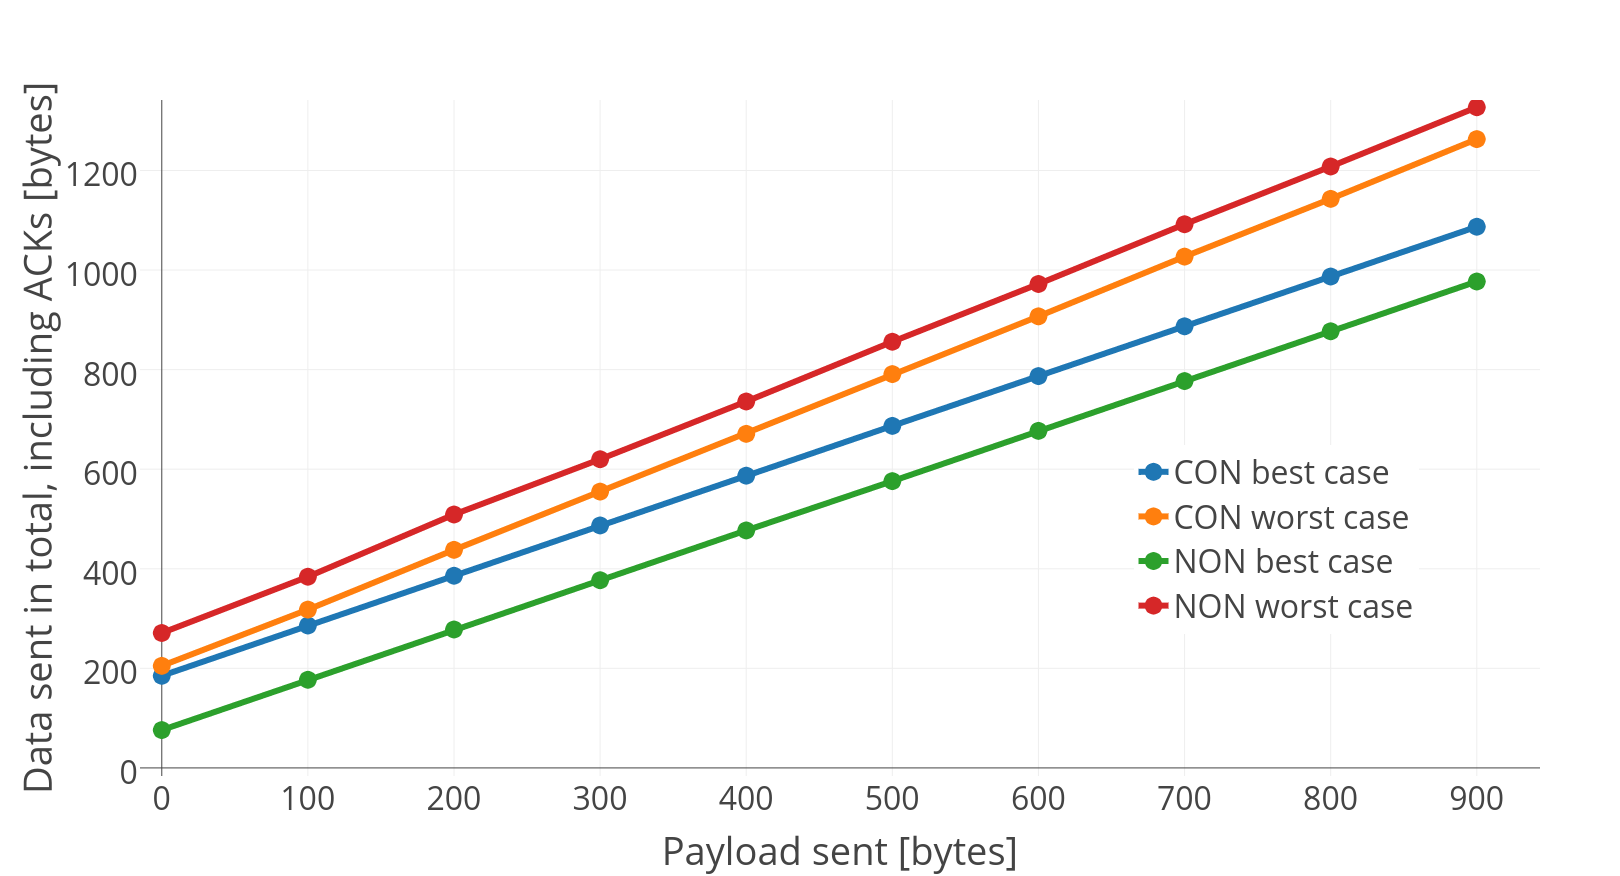
\includegraphics[width=1.0\textwidth]{bestCaseworstCase3.png}    
    \caption{Number of bytes per second}
    \label{fig:bestCaseworstCase}
\end{figure}

\noindent Still, as seen in figure \ref{fig:bestCaseworstCase}, this turns out not to always be the case. The figure shows best and worst case of how many bytes that needs to be sent to transfer a given number of \gls{payload}. For example, using \gls{non} it takes 576 byte to transfer 500 byte payload in best case, but 856 byte in worst case. This is because of the architecture of the two different versions of \gls{coap}. Even though \gls{non} does not require \glspl{ack}, underlying parts of the bluetooth architecture like \gls{acl} adds on some support for this. Also, to prevent a situation where the end node sends data forever without anyone receiving the data, \gls{ack} messages are still being sent regularly, approximately every 15th second in this network. This means, as shown in figure \ref{fig:bestCaseworstCase}, that \gls{non} \textit{normally} requires a lower amount of bytes to transport a given \gls{payload}, but in \textit{worst case scenario} it needs even more bytes than \gls{con}. 






\noindent The main question to comparison comes down to how often the worst case occurs in comparison to best case. Sending payload of 500 byte in both cases, \gls{non} results in most best case scenarios, while \gls{con} results in \textit{only} worst case scenarios. In specific numbers, this gives an average of \textit{598 bytes} sent for \gls{non}, and \textit{791 bytes}. This gives us the following equations to calculate how much of the total bytes sent that constitutes of the \gls{payload}. These calculations are based on measurements similar to the one shown in table \ref{coapNON700table} and \ref{coapCON700table}\footnote{The complete table containing the measurements can be found on \url{https://www.github.com/sische/MasterThesis/measurements}}. 



\begin{equation} \label{bestWorstEquation}
	\frac{500 \, byte \, payload}{\frac{791 \, bytes \,*\, 15 \, packets}{15}}\,*\,100 \% \approx 63,21 \%\, payload \, (CON)
\end{equation}

\begin{equation} \label{bestWorstEquation2}
\frac{500\, byte\, payload}{\frac{(576\, bytes\, *\, 13\, packets)\,+\,(856\, bytes\, *\, 2 \,packets)}{15}}\,*\,100 \% \approx 83,56 \%\, payload \, (NON)
\end{equation}

\noindent From these results it can be concluded that even though \gls{non} is considerably worse in worst case than \gls{con}, it is still needed about 20 \% less packets sent through the network to get the same amount of information through. This result is about the same as what was expected before the test. 



\section{Chapter summary}

\noindent In this chapter the most central experiments performed in the project have been presented and compared. The first problem up for discussion was if fragmentation of packets is a major issue in an \gls{iot} network like the network presented in this thesis. \Glspl{payload} from 0 to 1000 bytes were sent through the network, and the fragmented packets sent were being captured on the client side using Wireshark. The comparison between \gls{con} and \gls{non} shows both that there are very small differences between the two versions of the protocol, and that fragmentation of packets is not a major issue in such a network. 

\noindent The next experiments focused on \gls{goodput} in the system, the amount of data can be sent per second. \gls{con} is faster at small \glspl{payload}, mostly because this is requested by GET-requests. At approximately 500 bytes \gls{payload} \gls{con} start to use longer than 1 second to transfer, and is being bypassed by \gls{non}, which can send 600 bytes in one second. After this, both versions start to climb with approximately a rate of 1 second per 500 bytes of \gls{payload}. Comparisons to the capacity of the different technologies are being discussed, to find out that these results are much lower than expected. Another comparison experiment presented shows that between 500 and 900 bytes \gls{payload} in \gls{con}, while 600 bytes \gls{payload} is the optimal for \gls{non}. This gives a maximal \gls{goodput} of approximately 600 bytes/second. 

\noindent Because there are different additional protocols in the two versions of \gls{coap}, the amount of bytes sent in total through the network is not constant, even though the \gls{payload} is constant. Measurements show that \gls{non} require the least packets in best case, but also the most in worst case. Despite this, \gls{non} most of the time manages to stay on best case, giving it the best \% payload of all packets sent at 500 bytes, with 83,56 \% compared to 63,21 \% in \gls{con}.   


